\documentclass[a4paper,notitlepage]{report}

\usepackage[english]{babel}
\usepackage{mathtools, amsmath, booktabs}
\usepackage[makeroom]{cancel}
\usepackage[affil-it]{authblk}
\usepackage{braket}
\usepackage{hyperref}
\usepackage[english]{babel}
\usepackage{graphicx}
\usepackage{enumitem}
\usepackage{float}

\setlength\parindent{0pt}
\setlength{\parskip}{0.5em}

\makeatletter
    \def\thebibliography#1{\chapter*{References\@mkboth
      {REFERENCES}{REFERENCES}}\list
      {[\arabic{enumi}]}{\settowidth\labelwidth{[#1]}\leftmargin\labelwidth
	\advance\leftmargin\labelsep
	\usecounter{enumi}}
	\def\newblock{\hskip .11em plus .33em minus .07em}
	\sloppy\clubpenalty4000\widowpenalty4000
	\sfcode`\.=1000\relax}
    \makeatother

\begin{document}
\addtolength{\jot}{1em}


\title{Gravitational Solitons From Topology}
\author{Tasos Bouzikas\\
{\small Supervised by: Dr. Bert Vercnocke (UvA)}}
\affil{Department of Theoretical Physics, Faculty of Science\\
Utrecht University}
\date{}

\maketitle
\vspace{8em}

\begin{abstract}
\noindent In General Relativity (GR) the Kerr Black hole is the unique vacuum solution for	a given mass and angular momentum. In Supergravity (SUGRA), the low-energy limit	of string theory that extends GR, there is another mechanism that can support matter and that is the non-trivial topology of spacetime. Many ``black hole microstate geometries'' are known that are supported by cohomological fluxes on topological cycles in the geometry. This mechanism has been described recently, in detail, in terms of Komar integrals and a Smarr formula by Gibbons and Warner, in the context of five dimensional SUGRA. In this project I investigate this mechanism thoroughly initially in 4 dimensions and then in 10 dimension in the context of Type IIA superstring theory. Moreover, I extend this idea to asymptotically not-flat AdS spacetime.
\end{abstract}

%--------------------------------------------------------------------------------

\chapter*{Acknowledgements}
\begin{centering}
I would like to thank my supervisor Bert Vercnocke, for his guidance and his priceless help, during the last nine months. 
I would also like to thank my classmates for helping me through our discussions, and also for their valuable comments.
Finally, I want to thank Georgia, since without her nothing would have happened.
\end{centering}

\tableofcontents

\chapter{Introduction}

\section{Brief History of Black Holes}

In 1915, Albert Einstein presented the theory of General Relativity (GR), which constitutes one of the cornerstones of Theoretical Physics, since it entails a novel description of gravity (For a general review of General Relativity see   \cite{carroll2004spacetime,hartle2003gravity,schutz2009first,mcmahon2006relativity}). 

The load-bearing part of GR is of course the Einstein field equations:

\begin{align}\label{A}
R_{\mu\nu} - \frac{1}{2} g_{\mu\nu} R = T_{\mu\nu}
\end{align}

\vspace{0.5 em}
where $R_{\mu\nu}$ and $R$ are the Ricci tensor and Ricci scalar respectively, $g_{\mu\nu}$ is the metric and $T_{\mu\nu}$ is the stress-energy tensor.

The first solution of (\ref{A}) that was ever found was the so-called Schwarzschild black hole, which was discovered by Karl Schwarzschild in 1916. The geometry of this black hole, is the well-known Schwarzschild metric:

\begin{align} \label{B}
ds^2 = - \Big(1- \frac{2GM}{r} \Big) dt^2 + \Big(1- \frac{2GM}{r} \Big)^{-1} dr^2 + r^2 d\Omega^2_2
\end{align}

\vspace{0.5 em}
where $M$ is the ADM mass of the black hole. It worth mentioning that the ADM energy is a way of defining energy at the boundaries of an asymptotically flat spacetime. The above-mentioned solution describes an empty spacetime (i.e $T_{\mu\nu} = 0$) and it is completely characterised by its mass $M$. As it was shown later by Birkhoff, Schwarzschild black hole is the only spherically symmetric vacuum solution that exists. 

\begin{figure}[ht]
\centering
\includegraphics [width=0.6\textwidth]{blackhole}
\caption{The impact of a black hole to spacetime continuum.}
\label{Mtheory}
\end{figure}

The following years, more light was shed on the field of black holes. More specifically, Reissner and Nordstrom, found a charged black hole, completely characterised by its electric charge $Q$ \cite{reissner1916eigengravitation,nordstrom1918energy}, while Kerr found a non static black hole, which in turn is characterised by its angular momentum $J$ \cite{kerr1963gravitational}.

On top of that, there is the so-called ``No-hair conjecture'', and later ``No-hair theorem'', which states that in 4 dimensions a black hole can be fully described by these three  parameters $M$, $Q$, and $J$. The latter suggests that a solution which already contains these three parameters, is the most general solution that one could get in 4 dimensions. This solution is known as the ``Kerr-Newman'' black hole \cite{kerr1963gravitational,newman1965note,newman1965metric}.

Based on the above, one could speculate that there is nothing more general, concerning the parameters that you can use in order to describe a black hole, beyond Kerr-Newman black hole. However, after the emergence of string theory, and later superstring theory, the idea of black holes in higher dimensions arose. 

\section{New Solutions: Microstate Geometries}

Despite the fact that GR proved to be right in almost every experiment that has been done, a major drawback of the theory is that it fails to come to an agreement with quantum mechanics. However, the occurrence of black holes creates some famous paradoxes and then a quantum theory of gravity becomes really necessary in order to solve those paradoxes.

Two major aspects that involve black holes, and they appear to be of great importance, and at the same time difficult to solve, comprise of the famous ``Information Paradox'' and the ``Black hole entropy''. (For a general review of the paradoxes see   \cite{bena2008black,strominger1996microscopic,skenderis2000black}).

Concerning the ``Information Paradox'', it is widely known that an object that passes the event horizon of a black hole cannot escape the gravitational force of the black hole afterwards. To put it differently, every piece of information regarding these objects remains trapped into the black hole. However, Hawking provided evidence that it is possible for a virtual particle pair to be created near the horizon of a black hole, and furthermore, that even if one of them falls into the black hole, the other can still escape in form of a thermal radiations that carries no information, known as Hawking radiation. Eventually, this radiation will lead to the evaporation of the black hole and all the information that will have been inside the black hole, will be lost \cite{hawking1974black}. This process demolish the idea of unitarity evolution, and it is in contrast with quantum physics.

Regarding the second aspect, it was suggested by Bekenstein and Hawking in 1972, that a well-defined entropy of a black hole should be connected with its horizon area according to the following formula \cite{bekenstein1973black,hawking1974nature}.

\begin{align}
S_{\text{BH}} = \frac{A}{4G}
\end{align}

\vspace{0.5 em}
where $S$ is the entropy of the black hole and $A$ is the area of the event horizon. The nature of this entropy is purely thermodynamical. Our experience from classical physics, and more specifically from the principals of statistical mechanics, has taught us that the entropy has also a statistical nature which it must be related to a microscopic description of a black hole. We reverse the term ``microstate geometries'' for all the different microscopic descriptions of a black hole which they are also solutions to Einstein equations. Since a microstate geometry should exclude any entropy itself, it becomes apparent that the microstate geometry should be without horizon. Furthermore, another necessity of the microstate geometries is that they need to be smooth everywhere. That way, any potential naked singularities after removing the horizon will be kept away. On top of that we can also take for granted that the microstate geometries are time-independent. These properties reveal a solitonic nature of microstate geometries. 

Considering however, that a large horizon entails a large entropy, it is necessary to assume the existence of a very large number of possible microstate geometries. (According to Boltzmann's entropy formula there should be $e^S$ number of micorstate geometries). Inevitably, the question that emerges is how can we find such a big number of different microstate geometries. 

As it has been already stated above, an ideal quantum gravity theory needs to incorporate a solution for the paradoxes we described. String theory seems to provide the means for the solution of those problems, and consequently to become a successful quantum gravity theory. It was shown, that the correct number of microstate geometries that matches the Bekenstein-Hawking entropy \cite{bekenstein1973black,hawking1974nature}, can be obtained by counting the different configurations of the branes and strings in the zero gravitational coupling limit. Despite this progress however, the geometric aspects of the microstates, following the initiation of the gravitational coupling, still remain unsolved. 

\section{Conserved Charges}

In this section, we will describe a theoretical mechanism able to produce the parameters that can describe a black hole as conserved charges out of given solutions of black holes. (For a review see\cite{carroll2004spacetime,townsend1997black}). Motivated by the easiest of the parameters to be obtained, the electric charge, one can show that it can be interpreted as the associated conserved charge of a conserved current.

\subsection{Electric Charge - Electrodynamics}

Starting with Maxwell's equations written in terms of differential forms (see Appendix \ref{AB})\footnote{In this project we follow the conventions of \cite{danielsson2009towards}}.

\begin{align}
dF = 0 \qquad d*F = *j
\end{align}

\vspace{0.5 em}
where $F$ is the 2-form corresponding field strength of the 1-form $U(1)$ gauge field $A$, and $j$ is the current, it is very easy to prove that the resulting current is conserved, since:

\begin{align}
d*j = d^2 *F = 0
\end{align}

\vspace{0.5 em}
where the basic property of the exterior derivative $d^2=0$ has been used. 

In order to find the associated conserved charge, one has to integrate the conserved current over the spatial components of the manifold $\Sigma$ that the theory lives on:

\begin{align}
Q = \int\limits_{\Sigma} *j = \int\limits_{\Sigma} d*F = \int\limits_{\partial\Sigma} *F
\end{align}

\vspace{0.5 em}
where in the last equality Stokes' theorem was applied. The final integral stands for the integration of the dual field over a hyper-surface that includes the manifold $\Sigma$. This is what we is defined in the electrodynamics as the electric charge that is included in the area covered by the hyper-surface $\partial\Sigma$. Hence, the associated charge of the conserved current is the electric charge.

\subsection{Komar Integral}
 
In an effort to find a similar process able to produce the mass $M$ and the angular momentum $J$ as conserved charges, we attempt to define an 1-form current with components $j^\mu$ of the form \cite{carroll2004spacetime,townsend1997black}

\begin{align}
j^\mu = T^{\mu\nu} K_\nu 
\end{align}

\vspace{0.5 em}
where $T^{\mu\nu}$ is the stress energy tensor and $K^\mu$ is a Killing vector admitted by the geometry. It can be easily shown that this current is conserved, since:

\begin{align}
\nabla_\mu j^\mu = \nabla_\mu (K_\nu T^{\mu\nu}) = (\nabla_\mu K_\nu) T^{\mu\nu} + K_\nu (\nabla_\mu T^{\mu\nu}) = 0 
\end{align}

\vspace{0.5 em}
where in the last equality each individual term is zero, due to the Killing equation, the symmetries of $T^{\mu\nu}$, and also due to the fact that $T^{\mu\nu}$ is conserved itself.

One cannot avoid observing though, that a charge of the form:

\begin{align}
Q = \int\limits_{\Sigma} j^\mu d\Sigma_\mu = \int\limits_{\Sigma} T^{\mu\nu} K_\nu  d\Sigma_\mu
\end{align}

\vspace{0.5 em}
could create some problems. In the case of the Schwarzschild spacetime for example, where the stress-energy tensor vanishes everywhere, the above integral produces a zero charge, despite the fact that one anticipates to obtain a non-zero energy. As we already mentioned, there is a non-zero ADM energy, even in the Schwarzschild black hole. 

In order to overcome this problem, we define a new 1-form current with components $j^\mu$ of the form:

\begin{align} \label{C}
j^\mu = R^{\mu\nu} K_\nu 
\end{align}

\vspace{0.5 em}
The difference with the previous current is that now we use the Ricci tensor $R^{\mu\nu}$ instead of the stress-energy tensor. 

This new current is still conserved since:

\begin{align}
\nabla_{\mu} j^\mu &= \nabla_{\mu} (K_\nu R^{\mu\nu}) \\ \notag
& = (\nabla_{\mu}K_\nu) R^{\mu\nu} + K_\nu (\nabla_{\mu}R^{\mu\nu}) \\ \notag
& = \frac{1}{2} (\nabla_{\mu}K_\nu + \nabla_{\mu}K_\nu) R^{\mu\nu} + K_\nu \frac{1}{2} (\nabla^{\nu}R) = 0 
\end{align}

\vspace{0.5 em}
where the Killing equation, and Killing vector properties have been used.

Having removed the previous problems arose by a current that contains the stress-energy tensor, we are now able to find the conserved charge that results out of (\ref{C}). The conserved current (\ref{C}) can be written in terms of differential forms as $j = *dK$ where $K$ the Killing 1-form. Using this expression for the current, in the same manner as in electrodynamics, we can find the following associated charge:

\begin{align}
Q = \int\limits_{\Sigma} *j = \int\limits_{\Sigma} d*dK = \int\limits_{\partial\Sigma} *dK 
\end{align}

\vspace{0.5 em}
where $\Sigma$ is a space-like hyper-surface and $\partial\Sigma$ stands for the outer boundary of the space-like hyper-surface $\Sigma$. This final expression is called ``Komar integral'' \cite{komar1963positive}.

\begin{align}\label{D}
Q_{K} = \kappa_{D} \int\limits_{\partial\Sigma} *dK
\end{align}

\vspace{0.5 em}
where $\kappa_D$ is a normalisation constant that can be specified by linearising Einstein equations, and by assuming that at infinity the $T_{00}$ is the dominant term of the stress - energy tensor, i.e : $T_{00} \gg T_{0i},T_{ij}$ for $i,j \not= 0$. Under this energy condition, one can show \cite{gibbonsglobal}

\begin{align}
\kappa_{D} = - \frac{1}{16\pi G_{D}} \frac{D-2}{D-3}
\end{align}

\subsection{Example: The Schwarzschild Black Hole}

A way to verify that (\ref{D}) indeed produces the mass $M$ as the associated conserved charge, is to apply the formula on the Schwarzschild black hole \cite{carroll2004spacetime}.

As it was already mentioned, Schwarzschild black hole is a solution to the empty Einstein equation $R_{\mu\nu} = 0$. This solution has the form (\ref{B}). Since the metric is static, it admits a time-like Killing vector of the form $K^\mu = (1,0,0,0)$. We will calculate the Komar integral for the given geometry and Killing vector.

The Komar integral (\ref{D}) in 4 dimensions, in terms of indices is:

\begin{align}
Q_K = \frac{1}{4\pi G} \int\limits_{\partial\Sigma} d^2x \sqrt{\gamma^{(2)}} \sigma_\mu n_\nu \nabla^\mu K^\nu
\end{align}

\vspace{0.5 em}
where $\gamma$ is the metric at infinity, and $\sigma_\mu$,$n_\nu$ are the normal unit vectors of the huper-surface $\partial\Sigma$ normalised to $\sigma_\mu \sigma^\mu = -1$ and $n_\mu n^\mu = +1$.

For the normalised (unit) vectors we can show:

\begin{align}
n_\mu = \Big(1 - \frac{2GM}{r} \Big)^{-\frac{1}{2}} \delta^\mu_r \qquad \sigma_\mu = - \Big(1 - \frac{2GM}{r} \Big)^{\frac{1}{2}} \delta^\mu_t
\end{align}

\vspace{0.5 em}
Hence, the only surviving term in Komar expression is:

\begin{align} \label{3}
\sigma_\mu n_\nu \nabla^\mu K^\nu = \sigma_t n_r \nabla^t K^r = - \frac{GM}{r^2}
\end{align}

\vspace{0.5 em}
The metric at infinity is:

\begin{align}
\gamma^{(2)}_{ij} = r^2 (d\theta^2 + \sin^2\theta d\phi^2)
\end{align}

\vspace{0.5 em}
therefore

\begin{align}
\sqrt{\gamma^{(2)}} = r^2 \sin\theta
\end{align}

\vspace{0.5em}
Substituting back, we get:

\begin{align}
Q_K = \frac{1}{4\pi G} \int d\theta d\phi r^2 \sin\theta \Big( \frac{GM}{r^2} \Big) = M
\end{align}

\vspace{0.5 em}
As we can observe, the Komar integral is indeed the expected ADM mass. However, despite the fact that we proved that the Komar integral is equal to the mass only for the Schwarzschild case, it is true that Komar charge can always be interpreted as the mass. To elaborate on the latter, let us first, remind ourselves that the components of the conserved current $j$ are $R_{\mu\nu} K^\nu$ and the only non vanishing components of the Killing vector is the temporal one. Subsequently,  the only term that survives inside the Komar integral is the temporal component of the Ricci tensor $R_{00}$ which according to Einstein equations is equal to $T_{00}$. We neglected the contribution of the trace of the stress energy tensor, since as we already mentioned, the energy condition that we imposed, implies that at infinity $T_{00} \gg T{ij}$. The temporal component of the stress energy tensor can be interpreted as energy (or mass), hence we are always able to interpret the Komar integral as energy.


\section{Smarr Formula}

The Komar integral can be extended in such a way to include a topological term, as well as a term coming from the event horizon. (For a review see \cite{kodama2011lecture}). That way, it can be shown that the Komar mass, which is calculated at infinity, is comprised by a contribution coming from the bulk (i.e topology), and a contribution coming from the event horizon. 

The way to succeed that, is to consider a new kind of manifold that describes the spacetime (Figure \ref{Smarr}). In this new configuration, it is assumed that the space contains an inner boundary, apart from the boundary at infinity. Between those two boundaries there is the bulk of our space, that it might be empty or, as it will be shown in the next sections, filled with matter fields.

\begin{figure}[ht]
\centering
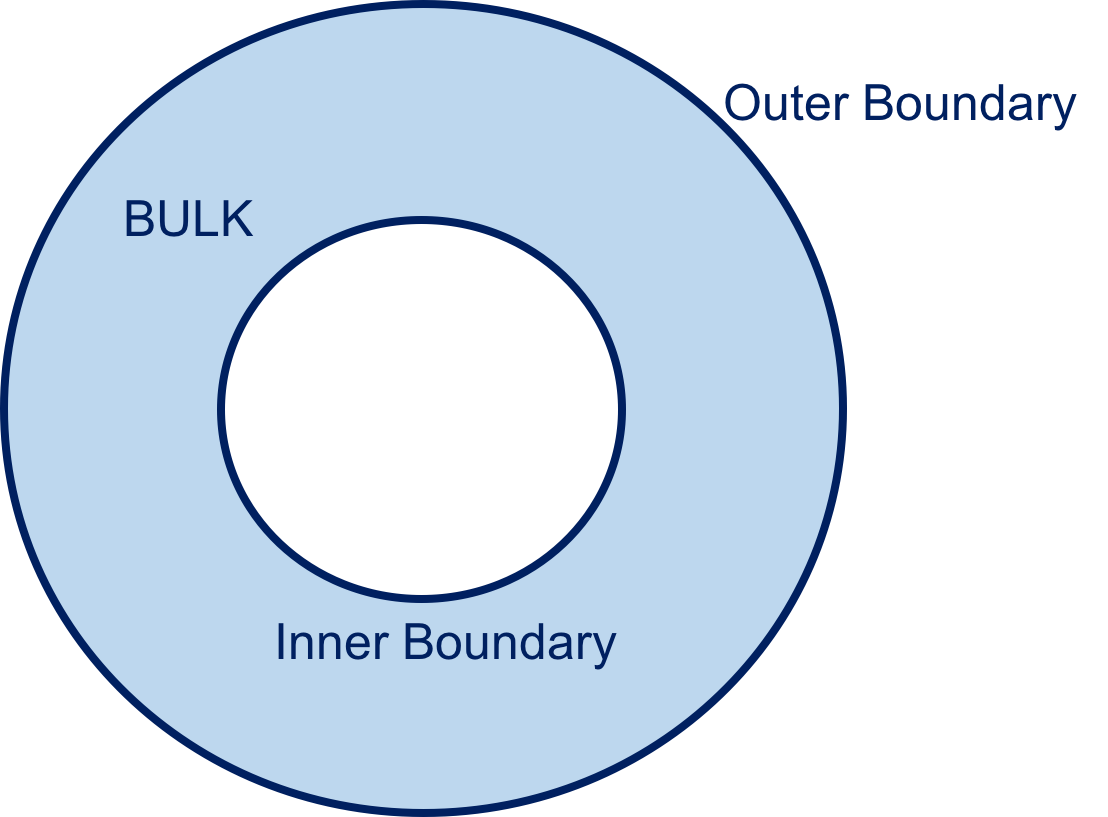
\includegraphics [width=0.5\textwidth]{Smarr}
\caption{A manifold with two boundaries: An outer boundary, an inner boundary and the bulk in-between.}
\label{Smarr}
\end{figure}

Regarding the integration of differential forms in such a space, Stokes' theorem for a manifold with two boundaries is of the form:

\begin{align}
\int\limits_{\Sigma} d A_{p} = \int\limits_{\partial \Sigma^{\text{out}}} A_{p} - \int\limits_{\partial \Sigma^{\text{int}}} A_{p}
\end{align}

\vspace{0.5 em}
Coming to our case, for the conserved current $j=*dK$, one obtains:

\begin{align} \label{G}
\int\limits_{\Sigma} d *dK &= \int\limits_{\partial \Sigma^{\text{out}}} *dK - \int\limits_{\partial \Sigma^{\text{int}}} *dK  
\end{align}

\vspace{0.5 em}
The first integral of the RHS of equation (\ref{G}) is the definition that we gave for the Komar integral. As a last step, in order to make connection with black holes, we identify the inner boundary of the manifold as the event horizon of a black hole. That way, our configuration consist of a black hole with its event horizon as an inner boundary, the bulk, and the outer boundary (Figure \ref{Smarr}). Finally, by rearranging terms we obtain:

\begin{align} \label{E}
Q_{K} = \int\limits_{\Sigma} d *dK + \int\limits_{\partial \Sigma^{\text{h}}} *dK
\end{align}

\vspace{0.5 em}
Equation (\ref{E}) is called ``Smarr Formula'', and it relates the Komar integral with contributions coming from the bulk, and from the event horizon \cite{smarr1973mass}. 

An application of the Smarr formula to the Schwarzschild black hole, leads to the definition of the Komar integral. Indeed, since the bulk of Schwarzschild spacetime is empty, the current, which is proportional to the Ricci tensor vanishes everywhere in the bulk. Hence, the topological term vanishes and the final expression we get is the original definition of the Komar integral. However, as we will show, there are also some other cases which can produce more interesting results.

It is used for the Smarr formula to be treated by assuming that there is no topology and  consequently, that all the contribution arises from the event horizon \cite{ross2005black}. In the previous section we already advocated that Komar integral can be interpreted as the ADM energy, and one could show that the integral at the event horizon is proportional to the area of the black hole covered by the hyper-surface of an event horizon. If we also include the other two parameters (electric charge and angular momentum) we will obtain that the contribution of the event horizon is also proportional to the electric charge and to the angular momentum. Hence, by ignoring topology, a manipulation of equation (\ref{E}) yields:

\begin{align} \label{F}
dE = \frac{\kappa}{8\pi} dA + \Omega dJ + \Phi dQ
\end{align}

\vspace{0.5 em}
where $\Omega$ is the angular velocity and $\Phi$ is the electrostatic potential. Equation (\ref{F}) is known as the first law of black hole thermodynamics \cite{kodama2011lecture}.

In this thesis we will treat the Smarr formula in a different way, namely by assuming that there is no event horizon and the whole contribution is coming from the bulk. We will also discuss how a mass can survive from collapsing in this horizonless case.

\section{Motivation and Aim of the Thesis}

In light of the foregoing, the aim of the present project is to study a mechanism which was originally created by Gibbons and Warner \cite{gibbonsglobal}, in four and ten dimensions. This mechanism shows, by making use of the Komar Integral and the Smarr Formula that has been described before, that one is able to measure a non-zero mass coming from the bulk of the spacetime, even without an event horizon. A black hole cannot exist without the existence of an event horizon, since in the absence of the latter what remains is a naked singularity absorbing everything. In this extreme case of no event horizon the whole universe would collapse into the singularity and in the end, a zero Komar mass would be admitted. However, as it was mentioned, one, using this new mechanism that we described, is able to obtain a non-zero mass, coming from a solution without an event horizon. These solutions are the microstate geometries that have already been discussed.

To begin with, we focus on  four dimensions, in which we clarify that topology makes it very hard to find such solutions. In particular, we will show that in four dimensions the final result depends only in the first cohomology group of the manifold (see Appendix \ref{ABC}). Therefore if we make the assumption that we work only with simply connected topological spaces which they admit a trivial first cohomology group, we will show that this trivial topology generates a non-interesting result which advocates the non-existence of solitons in four dimensions. That will underlie the need of introducing extra dimensions, which as we will show, provide us with more freedom on choosing the topology. Indeed, even for one extra dimensions of Gibbons and Warner \cite{gibbonsglobal}, one can observe that there is more than one cohomology groups evolved. In our project, more specifically, we work in frame of the ten dimensional supergravity \cite{freedman2012supergravity,nastase2011introduction}, which is the low energy limit of ten dimensional type II superstring theory.

Finally, we examine the validity of this mechanism under the existence of a cosmological constant $\Lambda$ which leads to either a deSitter or AdS spacetime, depending on its value. The cosmological constant $\Lambda$ creates a curvature which gives a divergent Komar integral. In this thesis, we will try to treat this divergence both at infinity, meaning the Komar mass, and in the bulk, by trying to cancel the divergence appearing in Smarr formula. As we see, there is a lot of literature concerning this topic In our project we will treat the problem by the use of a concept called ``Killing potential''  \cite{bazanski1990gauss,kastor2008komar}, since, as we will show, it an also be used in order to treat the divergence in the bulk, i.e in the RHS of Smarr formula.

%--------------------------------------------------------------------------------

\chapter{AdS Spacetime}

The main tools that will build the mechanism involving topology, that will be described in the next chapters, are the Komar integral and the Smarr formula. In the present chapter we examine the behaviour of these formulas under the presence of a non-zero cosmological constant $\Lambda$. That way, we show that the mechanism can be extended to AdS spacetime. In this project we will focus only on four-dimensional AdS spacetime, however, the manipulation that we will present works well in any number of dimensions.

\section{Komar Integral in AdS Spacetime}

The definition (\ref{D}) of the Komar integral does not take into account the curvature of the spacetime. In the current chapter we want to study the behaviour of Komar integral in a spacetime which also includes a negative cosmological constant $\Lambda$. This leads to curved AdS spacetime. Up to now we have been dealing with asymptotically flat spacetimes and as we will show, spacetime with a cosmological constant, produces a divergent Komar integral. This suggests that the Komar integral (\ref{D}) is not well-defined for spaces with curvature (For a more general review see\cite{bazanski1990gauss,kastor2008komar,kastor2009enthalpy}).

The Hilbert-Einstein action, including a cosmological constant in 4 dimensions is of the form:

\begin{align} \label{I}
\frac{1}{2\kappa} \int d^4x \sqrt{-g} \Big( R - 2\Lambda \Big)
\end{align}

\vspace{0.5 em}
The variation of the action with respect to the metric yields:

\begin{align}\label{H}
R_{\mu\nu} - \frac{1}{2} g_{\mu\nu} R + \Lambda g_{\mu\nu} = 0
\end{align}

\vspace{0.5 em}
By contraction of the indices we get straightforwardly that $R=4\Lambda$, and by substituting back to (\ref{H}) we obtain:

\begin{align} \label{W}
R_{\mu\nu} = \Lambda g_{\mu\nu}
\end{align}

\vspace{0.5 em}
Since the Komar integral depends on the Ricci tensor, we can very easily conclude that it is proportional to the integral of the cosmological constant. Subsequently, the charge is proportional to the volume of the spacetime, and thus, since the integration takes place at infinity, the radius goes to infinity and the Komar integral diverges.

In order to find explicitly the cause of this divergence, we will calculate the Komar integral for AdS spacetime. Following the same procedure as in the Schwarzschild black hole, the only ingredients that are needed, are a geometry that solves (\ref{W}) and a time-like Killing vector. Such geometry is the familiar $AdS_4$ spacetime, described by the following metric

\begin{align} \label{Z}
ds^2 = - \frac{r^2}{R^2} dt^2 + \frac{R^2}{r^2} dr^2 + r^2 d\Omega^2_2
\end{align}

\vspace{0.5 em}
where in abstract dimensions

\begin{align} \label{Z}
\frac{1}{R^2} = \frac{2\Lambda}{(D-1)(D-2)}
\end{align}

\vspace{0.5 em}
where D is the number of dimensions of spacetime. In our case for $D=4$ we get $\frac{1}{R^2} = \frac{\Lambda}{3}$.

Once again, the metric does not depend on time, hence, it admits a time-like Killing vector of the form $K^\mu = (1,0,0,0)$. Repeating the same steps as before, one obtains for the Komar integral

\begin{align} \label{Y}
Q_{K} = \int\limits_{\partial\Sigma}*dK = \int\limits_{\partial\Sigma} d\Sigma_{\mu\nu} \nabla^\mu K^\nu = \int\limits_{\partial\Sigma} d\Sigma_{tr} \frac{r}{R^2}
\end{align}

\vspace{0.5 em}
As we can observe, the integral is proportional to the radius, hence, for $r \rightarrow \infty$, the charge also goes to infinity. This entails that the original definition of Komar integral is not well defined in the case of an asymptotically AdS spacetime. 

\section{Possible Solutions For the Divergence}

\subsection{Various Solutions}

There is a lot of literature concerning the divergent Komar integral for AdS spacetime. For instance, Brown and York proposed the idea of the quasilocal stress-energy tensor, which is a redefinition of the latter at infinity, including the extrinsic curvature of the spacetime $\Theta$ as

\begin{align}
T^{\mu\nu}_{\text{bound}} = \frac{1}{8\pi G} \Big( \Theta^{\mu\nu} - \Theta \gamma_{\mu\nu} + \frac{2}{\sqrt{-\gamma}} \frac{\delta S_{\text{ct}}}{\delta \gamma_{\mu\nu}} \Big)
\end{align}

\vspace{0.5 em}
where $S_{\text{ct}}$ is an extra counter-term that cancels the divergency coming from the curvature \cite{brown1993quasilocal,balasubramanian1999stress}. It worth mentioning that indeed, one can show that this idea can treat the problem of divergence in pure AdS spacetimes, however it does not apply well in spacetimes of the form $AdS_p \times S_q$. Despite the fact that such spaces are flat, since the negative curvature of AdS is exactly cancelled by the positive curvature of the sphere, the Komar integral still diverges at infinity. 

Another way to treat the problem could be via gravitational Hamiltonian formalism, introduced by Hawking and Horowitz \cite{hawking1996gravitational}. It needs to be mentioned though, that this is a much more general framework, which can be used also in our case.

However, in this present project, we will try to fix the divergence using the Killing potential, which was first introduced in \cite{bazanski1990gauss,kastor2008komar}. The reason why we chose the Killing potential is because it also fits well with the divergence coming from the cosmological constant in the bulk.

\subsection{Killing Potential}

In this section we introduce the Killing potential $\omega^{\mu\nu}$, and we show how it can be used in order to treat the divergence coming from $\Lambda$ \cite{kastor2008komar,kastor2009enthalpy}.

Let us first try to define it. A Killing vector is the solution of the Killing equation:

\begin{align} \label{N}
\nabla_{\mu} K_{\nu} + \nabla_{\nu} K_{\mu} = 0
\end{align}

\vspace{0.5em}
or by contracting the indices:

\begin{align} \label{M}
\nabla_{\mu} K^{\mu} = 0
\end{align}

\vspace{0.5em}
Motivated by equation (\ref{M}) we define the fully antisymmetric Killing potential $\omega^{\mu\nu}$ in such a way so that the derivative of the Killing potential is equal to the Killing vector

\begin{align} \label{O}
K^\nu = \nabla_\mu \omega^{\mu\nu}
\end{align}

\vspace{0.5em}
Acting with a derivative on the last equation, we observe that the symmetric part of the derivatives combined with the antisymmetric Killing potential, satisfies equation (\ref{M})

\begin{align} \label{5}
\nabla_\mu K^\mu = \nabla_\mu \nabla_\nu \omega^{\nu\mu} = 0
\end{align}

\vspace{0.5em}
It worth mentioning that the Killing potential is not uniquely defined, since we can always add an exact term of the form $\nabla_\rho \lambda^{\rho\mu\nu}$ and the new Killing potential $\tilde{\omega}_{\mu\nu} = \omega_{\mu\nu} + \nabla_\rho \lambda^{\rho\mu\nu}$ satisfies again equation (\ref{M}).

As far as the divergence is concerned, the main idea is to use the Killing potential as a counter-term that we will add to the original Komar integral definition (\ref{D}), hoping that it will consequently cancel the divergence coming from the cosmological constant.

The new, redefined, Komar integral for asymptotically non-flat spacetimes using the Killing potential, in abstract dimensions, will be of the form:

\begin{align} \label{M1}
Q_K = \int\limits_{\partial\Sigma} d\Sigma_{\mu\nu} \Big( \nabla^\mu K^\nu + \frac{2\Lambda}{D-2} \omega^{\mu\nu} \Big)
\end{align}

\vspace{0.5em}
This redefinition can be seen as a generalisation of the Komar integral. In the case of a non-AdS spacetime, the cosmological constant vanishes and we get the original definition of the Komar integral(\ref{D}).

For the abstract dimensional AdS$_D$ spacetime geometry (\ref{Z}) and a Killing vector of the form $K^\mu = (1,0,0,0)$, we can solve equation (\ref{O}). By assuming that Killing potential does not depend on the angles, we can show that the only surviving term in D dimensions is:

\begin{align} \label{M2}
\omega^{rt}_{\text{AdS$_D$}} = -\omega^{tr}_{\text{AdS$_D$}} = \frac{r}{D-1}
\end{align}

\vspace{0.5 em}
Let us apply equations (\ref{M1}) and (\ref{M2}) to our 4 dimensional problem. For $D=4$ (\ref{M1}) becomes

\begin{align} 
Q_K = \int\limits_{\partial\Sigma} d\Sigma_{\mu\nu} \Big( \nabla^\mu K^\nu + \Lambda \omega^{\mu\nu} \Big)
\end{align}

\vspace{0.5em}
while (\ref{M2}) is simply

\begin{align} 
\omega^{rt}_{\text{AdS$_4$}} = -\omega^{tr}_{\text{AdS$_4$}} = \frac{r}{3}
\end{align}

\vspace{0.5em}
Hence, by taking into consideration the redefined Komar integral (\ref{O}), and the result we obtained for the original Komar integral \ref{Y} we get

\begin{align}
Q_{K} &= \int\limits_{\partial\Sigma} d\Sigma_{tr} \Big( \frac{r}{R^2} + \Lambda \omega^{tr} \Big) \\ \notag
&= \int\limits_{\partial\Sigma} d\Sigma_{tr} \Big( \frac{\Lambda r}{3} - \Lambda  \frac{r}{3} \Big) \notag \\
& = 0
\end{align}

\vspace{0.5 em}
As we can see, the divergence at infinity is cancelled due to the contribution coming from $\omega^{\mu\nu}$ and yields $Q_K = 0$. However, one is still able to interpret the charge as the mass from the remaining stress energy tensor of Einstein equations. To elaborate more on that, the same procedure can be applied to AdS-Schwarzschild geometry. In that case, Killing Potential will treat the divergence coming from the AdS part of the metric, and the remaining Schwarzschild part will produce the non-zero mass.

We should mention once again that this procedure works fine for any number of dimensions.

\section{Smarr Formula \& Killing Potential}

Smarr formula (\ref{E}) can be written in terms of indices in the following way

\begin{align} \label{X}
Q_{K} =\int\limits_{\Sigma} R^{\mu\nu} K_\nu d\Sigma_{\mu} + \int\limits_{\partial \Sigma^{\text{h}}} \nabla^{\mu} K^{\nu} d\Sigma_{\mu\nu}
\end{align}

\vspace{0.5em}
As we showed in the previous section, after including the Killing potential term, the Komar integral does not diverge. That means that the LHS of (\ref{X}) is finite, hence one would expect that the RHS is also free of divergences.

In order to show this, we first have to add the Killing potential inside the two integrals. To begin with the horizon term integral, we add $\omega_{\mu\nu}$ in the same way as we did for the outer boundary integral.  On the other hand, in order to add $\omega_{\mu\nu}$ in the bulk one has to use Stokes' theorem, since it is not a boundary term. The Smarr formula after adding the extra terms becomes

\begin{align} \label{T}
Q_{K} = \int\limits_{\Sigma} \Big( R^{\mu\nu} K_\nu + \Lambda \nabla_\nu \omega^{\mu\nu} \Big) d\Sigma_{\mu} + \int\limits_{\partial \Sigma^{\text{h}}} \Big( \nabla^{\mu} K^{\nu} + \Lambda \omega^{\mu\nu} \Big) d\Sigma_{\mu\nu}
\end{align}

\vspace{0.5em}
In order to manipulate the second integral, one should know the geometry of spacetime around the event horizon, and then to solve equation (\ref{O}) for this specific geometry. However, as we already pointed out, in the end we will not contain an event horizon and this particular integral will vanish. Hence, there is no need to manipulate it more. The reason why we have not removed it yet, is because there are also some other terms that eventually will be moved there.

Concerning the bulk integral however, we must show that it is free of divergences. Indeed, by making use of the definition of the Killing potential (\ref{O}) and by substituting $R_{\mu\nu}$ from (\ref{W}) we get for the first integral of (\ref{T})

\begin{align}
Q_K &= \int\limits_{\Sigma} \Big( R^{\mu\nu} K_\nu + \Lambda \nabla_\nu \omega^{\mu\nu} \Big) d\Sigma_{\mu} \notag\\
&= \int\limits_{\Sigma} d\Sigma_{\mu} \Big( \Lambda K^\mu - \Lambda K^\mu \Big) \notag \\
&= 0 
\end{align}

\vspace{0.5 em}
As we can observe the result is consistent with the one we got for the Komar integral in the previous section. Hence, as we argued before, the Killing potential treats the divergence both at infinity and in the bulk, while remains unknown the impact of it in the horizon integral.

In the following chapters we will take for granted that we already dealt with the problem that arose from cosmological constant and we will not include it into our manipulations. The same will hold also for the Smarr formula which now takes the final form

\begin{align} \label{Smarr}
Q_{K} = \int\limits_{\Sigma} R^{\mu\nu} K_\nu d\Sigma_{\mu} + \int\limits_{\partial \Sigma^{\text{h}}} \Big( \nabla^{\mu} K^{\nu} + \Lambda \omega^{\mu\nu} \Big) d\Sigma_{\mu\nu}
\end{align}

%------------------------------------------------------------------------------------------

\chapter{Matter Fields}

Up to this point we have only considered empty spacetimes. However, the interesting part is to study the contribution coming form the bulk of a non-empty spacetime to the Komar mass. More specifically, since we are interested in horizonless solutions, we seek a non-vanishing Komar mass where the whole contribution will arise from the topology.

For that reason, we assume the existence of a vector multiplet of scalar fields $X^{I}$, as well as a vector multiplet of $U(1)$ gauge fields $A^I$ with their corresponding 2-form gauge field strengths $F^{I} = dA^I$, where $I$ counts the number of the fields. The reason why we use supergravity multiplets is twofold. First of all supergravity provides us with a framework in which we are able to perform calculations. Second, supergravity, as we will see in the next chapter, is the low energy limit of superstring theory, which will be the main topic of the next chapter \cite{freedman2012supergravity,nastase2011introduction}.

\section{The Action in Four Dimensions}

The starting point is the four dimensional Hilbert-Einstein action, including also a Klein-Gordon part for the scalar fields, and a Maxwell part for the gauge fields. The full action is of the form:

\begin{align} \label{3.1}
S = \int d^4x \sqrt{-g} \Big( R - \frac{1}{2} Q_{IJ} \partial_\mu X^I \partial^\mu X^J - \frac{1}{4} Q_{IJ} F^I_{\mu\nu} F^{J\mu\nu} - \frac{1}{4} C_{IJ} F^I_{\mu\nu} F^J_{\rho\sigma} \bar\epsilon^{\mu\nu\rho\sigma} \Big)
\end{align}

\vspace{0.5 em}
where both $Q_{IJ}(X)$ and $C_{IJ}(X)$ are functions of the scalar fields $X^I$. The cosmological constant is absent, since we already discussed the way to overcome the divergence. The $\bar\epsilon$ notation, means that this term does not contain the metric.

The last term of action (\ref{3.1}), the Chern-Simons term, does not contain the metric at all, hence is purely topological and it produces a topological current. We can make this clear, by focusing only on the part of the action that includes the gauge fields. This part may be rewritten using differential forms as (see Appendix \ref{ABC1})

\begin{align} \label{3.2}
S_{\text{gauge}} = - \int \Big( \frac{1}{2} Q_{IJ} *F^I \wedge F^J + C_{IJ} F^I \wedge F^J \Big)
\end{align}

\vspace{0.5 em}
Since $F^I = dA^I$ we get straightforwardly the Bianchi identity for the field strength which is
\begin{align} \label{3.3}
dF^I = 0
\end{align}

\vspace{0.5 em}
By varying the action with respect to the gauge field (see Appendix  \ref{ABC2}) we obtain the equation of motion for $F^I$ 

\begin{align} \label{3.4}
d(Q_{IJ} * F^J ) = *J_{CS} = - 2 d(C_{IJ}) F^J 
\end{align}

\vspace{0.5 em}
The RHS of this equation is the topological current $*J_{CS}$ produced by the Chern-Simons term.

At this point, it is a common procedure to define the dual field strength of $F^I$ to be the 2-form 

\begin{align} \label{3.5}
G_I = Q_{IJ} *F^J 
\end{align}

\vspace{0.5 em}
Since the Bianchi identity of the dual field is the equation of motion of the original fields, it follows trivially from (\ref{3.4}) that $G_I$ satisfies the following Bianchi identity

\begin{align} \label{3.6}
dG_I = - 2 d(C_{IJ}) F^J 
\end{align}

\section{Einstein Equations}

Our goal is to find the contribution from the bulk to the Komar mass. This can be done by calculating Smarr formula for the given action (\ref{3.1}). 

Smarr formula (\ref{Smarr}) in four dimensions is of the form

\begin{equation}\label{3.7}
M = \frac{1}{8\pi G_{4}} \int\limits_{\Sigma} R^{\mu\nu} K_{\mu} d\Sigma_{\nu} + \frac{1}{8\pi G_{4}} \int\limits_{\partial \Sigma^{\text{h}}} \Big( \nabla^{\mu} K^{\nu} + \Lambda \omega^{\mu\nu} \Big) d\Sigma_{\mu\nu}
\end{equation}

\vspace{0.5 em}
In order to calculate the Ricci tensor we vary the action (\ref{3.1}) with respect to the metric $g_{\mu \nu}$ and we obtain the following Einstein equations (see Appendix  \ref{ABC3})

\begin{align}\label{3.8}
R_{\mu\nu} - \frac{1}{2} g_{\mu\nu}R &= \frac{1}{2} Q_{IJ} \partial_{\mu} X^I \partial_{\nu} X^J - \frac{1}{4} Q_{IJ} g_{\mu\nu} \partial_{\rho} X^I \partial^{\rho} X^J + \frac{1}{2} Q_{IJ} F^I_{\mu\rho} F^{J\rho}_\nu \notag\\
& - \frac{1}{8} Q_{IJ} g_{\mu\nu}  F^{I}_{\rho\sigma} F^{J\rho\sigma}
\end{align}

\vspace{0.5 em}
By contracting the indices, keeping in mind that the fully contracted metric is equal to the dimensions of the space, we get for the Ricci scalar

\begin{align}\label{3.9}
R = \frac{1}{2} Q_{IJ} \partial_{\mu} X^I \partial^{\mu} X^J
\end{align}

\vspace{0.5em}
Substituting (\ref{3.9}) back into Einstein equations (\ref{3.8}) we get

\begin{align} \label{3.10}
R_{\mu\nu} = \frac{1}{2} Q_{IJ} \partial_{\mu} X^I \partial_{\nu} X^J + \frac{1}{2} Q_{IJ} F^I_{\mu\rho} F^{J\rho}_\nu - \frac{1}{8} Q_{IJ} g_{\mu\nu}  F^{I}_{\rho\sigma} F^{J\rho\sigma}
\end{align}

\vspace{0.5em}
Using the definition of the dual field (\ref{3.5}), we can prove the following relation between $F^I$ and $G^I$

\begin{align} \label{3.11}
Q^{IJ} G_{I\mu\rho} G_{J\nu}^\rho = Q_{KL} \Big(F^K_{\mu\rho} F^{L\nu\rho} - \frac{1}{2} g_{\mu\nu} F^K_{\rho\sigma} F^{L\rho\sigma} \Big)
\end{align}

\vspace{0.5em}
or by solving with respect to the metric:

\begin{align} \label{3.12}
g_{\mu\nu} Q_{IJ} F^I_{\rho\sigma} F^{J\rho\sigma} = 2 Q_{KL} F^K_{\mu\rho} F^{L\nu\rho} - 2 Q^{KL} G_{K\mu\rho} G_{L\nu}^\rho 
\end{align}

\vspace{0.5em}
By substituting (\ref{3.12}) back to (\ref{3.10}), we can rewrite the Ricci tensor in an elegant form, as a function of the derivatives of the scalar fields $X^I$ and the field strengths $F^I$ and $G_I$ as

\begin{align} \label{3.13}
R_{\mu\nu} = \frac{1}{2} Q_{IJ} \partial_{\mu} X^I \partial_{\nu} X^J + \frac{1}{4} Q_{IJ} F^I_{\mu\rho} F^{J\rho}_\nu + \frac{1}{4} Q^{IJ} G_{I\mu\rho} G^\rho_{J\nu}
\end{align}

\vspace{0.5 em}
Hence, the Smarr formula (\ref{3.7}) becomes

\begin{align} \label{3.14}
M =& \frac{1}{32\pi G_{4}} \int\limits_{\Sigma} \Big(2 Q_{IJ} K^\mu \partial_{\mu} X^I \partial^{\nu} X^J + Q_{IJ} K^\mu F^I_{\mu\rho} F^{J\rho\nu} + Q^{IJ} K^\mu G_{I\mu\rho} G^{\rho\nu}_{J} \Big) d\Sigma_\nu \notag\\
&+ \frac{1}{8\pi G_{4}} \int\limits_{\partial \Sigma^{\text{h}}} \Big( \nabla^{\mu} K^{\nu} + \Lambda \omega^{\mu\nu} \Big) d\Sigma_{\mu\nu}
\end{align}

\section{Invariances}

In order to be able to proceed, we need to calculate the contraction of the Killing vector with the derivative of the scalar fields, and the two field strengths. At this point, motivated by the fact that all the fields are time-independent, we make the assumption that the matter fields respect the symmetries of the metric. 

As it is known, if a spacetime admits a Killing vector $K$ then the Lie derivative of the metric vanishes

\begin{align} \label{3.15}
\mathcal{L}_{K} g_{\mu\nu} = 0
\end{align}

\vspace{0.5em}
Under the assumption that matter fields respect the isometries we get the following equations:

\begin{align} 
\mathcal{L}_{K} X^I = 0 \label{3.16}\\
\mathcal{L}_{K} F^I = 0 \label{3.17} \\
\mathcal{L}_{K} G_I = 0 \label{3.18}
\end{align}

\vspace{0.5em}
Using ``Cartan's magic formula'', the Lie derivative of a $p$-form is given by the following expression

\begin{align} \label{3.19}
\mathcal{L}_{K} \omega = d(i_{K} \omega_p)  + i_{K} d\omega_p
\end{align}

\vspace{0.5 em}
where the notation $i_{K}\omega_p$ stands for the contraction of the Killing vector with the first component of the p-form $\omega$. In terms of forms, it can be seen as a $(p-1)$-form.

Applying Cartan's magic formula (\ref{3.19}) on equation (\ref{3.16}) we obtain for the scalar fields

\begin{align}\label{3.20}
d(i_{K} X^I )  + i_{K} (d X^I) = 0
\end{align}

\vspace{0.5em}
where by definition $i_{K} X^I$ is zero since scalar fields do not carry any index in order to be contracted with the Killing vector. Hence, the final result is

\begin{align}\label{3.21}
i_{K} (d X^I) = 0
\end{align}

\vspace{0.5em}
which in terms of indices can be written as $K^\mu \partial_\mu X^I = 0$, which is the term appearing inside the Smarr formula (\ref{3.14}). Thus, the scalar fields do not contribute at all to the Komar mass and the whole contribution is coming from the gauge fields.

Since we can remove scalar fields form Smarr formula, equation (\ref{3.14}) can be rewritten in a more convenient way in terms of differential forms as

\begin{align} \label{3.22}
M =& \frac{1}{32\pi G_{4}} \int\limits_{\Sigma} \Big( Q_{IJ} i_{K}F^I \wedge * F^{J} + Q^{IJ} i_{K} G_{I} \wedge * G^J \Big) \notag\\
&+ \frac{1}{8\pi G_{4}} \int\limits_{\partial \Sigma^{\text{h}}} \Big( \nabla^{\mu} K^{\nu} + \Lambda \omega^{\mu\nu} \Big) d\Sigma_{\mu\nu}
\end{align}

\vspace{0.5 em}
or by using the dual field (\ref{3.5})

\begin{align} \label{3.23}
M &= \frac{1}{32\pi G_{4}} \int\limits_{\Sigma} \Big( i_{K}F^I \wedge G_I - i_{K} G_{I} \wedge F^I \Big) \\ \notag
&+ \frac{1}{8\pi G_{4}} \int\limits_{\partial \Sigma^{\text{h}}} \Big( \nabla^{\mu} K^{\nu} + \Lambda \omega^{\mu\nu} \Big) d\Sigma_{\mu\nu}
\end{align}

\vspace{0.5 em}
Equation (\ref{3.17}) for the Lie derivative of the field strength $F^I$, yields

\begin{align} \label{3.24}
d(i_{K} F^I)  + i_{K} (dF^I) = 0 \notag\\
d(i_{K} F^I) = 0  \notag\\
i_{K} F^I = \Lambda^I + d\lambda^I
\end{align}

\vspace{0.5em}
where in the second equality we used the Bianchi identity (\ref{3.3}) for $F^I$.

In (\ref{3.24}), $\Lambda^I$ is a closed but not exact 1-form, while $d\lambda^I$ is an exact 1-form, where $\lambda^I$ is a just a function.

Finally, the last equation (\ref{3.18}) admits for $G_I$

\begin{align} \label{3.25}
d(i_{K} G_I) &= - i_{K} (dG_I) = -  i_{K} (- 2 dC_{IJ} F^J) = 2 \Big( (i_{K}dC_{IJ}) F^J - dC_{IJ}  (i_{K}F^{J}) \Big)  \notag\\
&= -2 \Big( dC_{IJ} \wedge (\Lambda^J + d\lambda^J) \Big) = d \Big( -2C_{IJ} \wedge (\Lambda^J + d\lambda^J) \Big)
\end{align}

\vspace{0.5em}
where we made use of the Bianchi identity of $G_I$ field (\ref{3.6})
Finally, we get:

\begin{align} \label{3.26}
i_{K} G_I = -2C_{IJ} \Lambda^J - 2C_{IJ} d\lambda^J + H_{I} + dh_{I}
\end{align}

\vspace{0.5em}
where, as before, $H_{I}$ are closed but not exact 1-form and $h_{I}$ is a function. As we can observe, beside the harmonic and the exact part, the solution for $G_I$ contains also a term which is originated by the topological Chern-Simons current.

We point out, that in order for $\Lambda^I$ and $H_I$ to exist, one needs to make the assumption that the first cohomology group of the theory is non-trivial, i.e $H^1(M) \not= 0$.

It is also of great importance to distinguish between harmonic (as $\Lambda^I$ and $H_{I}$) and exact forms (as $\lambda^I$ and $h_{I}$) . The exact forms do not contribute at all to the the bulk integral, since they can be moved at the boundary integral by making use of Stokes theorem. On the other hand, harmonic forms, cannot be written as the exterior derivative of other forms, therefore, they contribute to the bulk.

\section{Smarr Formula}

In the previous section we calculated all the terms in Smarr formula, therefore by substituting (\ref{3.24}) and (\ref{3.26}) to (\ref{3.23}) we obtain

\begin{align} \label{3.27}
M =& \frac{1}{32\pi G_{4}} \int\limits_{\Sigma} \Big( (\Lambda^I + d\lambda^I)  \wedge (G_I + 2C_{IJ} \wedge F^J ) - (H_{I} + dh_{I}) \wedge F^I \Big) \notag\\
&+ \frac{1}{8\pi G_{4}} \int\limits_{\partial \Sigma^{\text{h}}} \Big( \nabla^{\mu} K^{\nu} + \Lambda \omega^{\mu\nu} \Big) d\Sigma_{\mu\nu}
\end{align}

\vspace{0.5 em}
One can verify, using the Bianchi identities that the expressions $(G_I + 2C_{IJ} \wedge F^J)$ and $F^I$ appearing in the bulk integral are closed. Motivated by that we can rewrite (\ref{3.27}) as

\begin{align} \label{3.28}
M =& \frac{1}{32\pi G_{4}} \int\limits_{\Sigma} \Big( \Lambda^I \wedge (G_I + 2C_{IJ} \wedge F^J ) - H_{I} \wedge F^I \notag\\
& \:\:\:\:\:\:\:\:\:\:\:\:\:\:\:\:\:\:\:\: + d(\lambda^I \wedge (G_I + 2C_{IJ} F^J)) - d(h_{I} \wedge F^I) \Big) \notag\\
&+ \frac{1}{8\pi G_{4}} \int\limits_{\partial \Sigma^{\text{h}}} \Big( \nabla^{\mu} K^{\nu} + \Lambda \omega^{\mu\nu} \Big) d\Sigma_{\mu\nu}
\end{align}

\vspace{0.5 em}
By making use of Stokes theorem we can move the exact terms of the bulk integral at the boundaries. At this point we make the assumption that the terms inside the derivatives are sufficiently small at infinity, thus, they do not affect the integral at infinity, and subsequently, the Komar mass.

As a final step, we assume that our solutions carry no event horizon, hence the horizon integral in Smarr formula vanishes, and the final result is of the form

\begin{align} \label{3.29}
M =& \frac{1}{32\pi G_{4}} \int\limits_{\Sigma} \Big( \Lambda^I \wedge (G_I + 2C_{IJ} \wedge F^J ) + F^I \wedge H_{I}   \Big)
\end{align}

\vspace{0.5 em}
Equation (\ref{3.29}) carries  highly important information. We can measure a non-zero mass coming out from a geometry that contains no event horizon. On top of that, it is time-independent, and in order to avoid any catastrophic collapses out of the fact that it is horizonless, it should also be regular everywhere. We believe that these solutions are the microstate geometries.

Of course, in order for (\ref{3.29}) to be non-zero, one has to impose a non-trivial first cohomology group. For trivial cohomology, all the closed forms are exact, meaning that harmonic forms are supported. Subsequently, $\Lambda^I_1 =0$ and $H_{I1}=0$, which leads us to observe that no topological contribution takes place. An obvious way to avoid this non interesting case is to focus on topological spaces with non-trivial first cohomology. However, if one restricts themselves to simply connected topological spaces, a trivial cohomology will be inevitable. This result was already known, since it was proved in a different way in \cite{breitenlohner19884}.

The only way to work with simply connected topological spaces and get a non-zero mass from the bulk, is by adding extra dimensions, as it has already been shown in the original work in five dimensions by Gibbons and Warner. The latter is analysed in the context of the ten-dimensional SUGRA, in the next chapter.

%----------------------------------------------------------------------------------------------------

\chapter{Type IIA Superstring Theory}

\section{Brief History of Superstring Theory }

Bosonic string theory requires 26 dimensions in order to be Lorentz invariant \cite{becker2006string,demystified2009demystified,green1987superstring,polchinski1998string2,polchinski1998string,schwarz2001introduction}. Supersymmetry, the symmetry that relates bosons to fermions, can drop the number of dimensions down to 10, and the theory that results is called superstring theory. 

During the early years of string theory, physicists developed several different types of formulation of string theory. In total, 5 different types have been developed: Type I, Type IIA, Type IIB, SO(32) Heterotic and $E_8\times E_8$ Heterotic. (Figure \ref{Mtheory})

\vspace{1.5em}

\begin{figure}[h!]
\centering
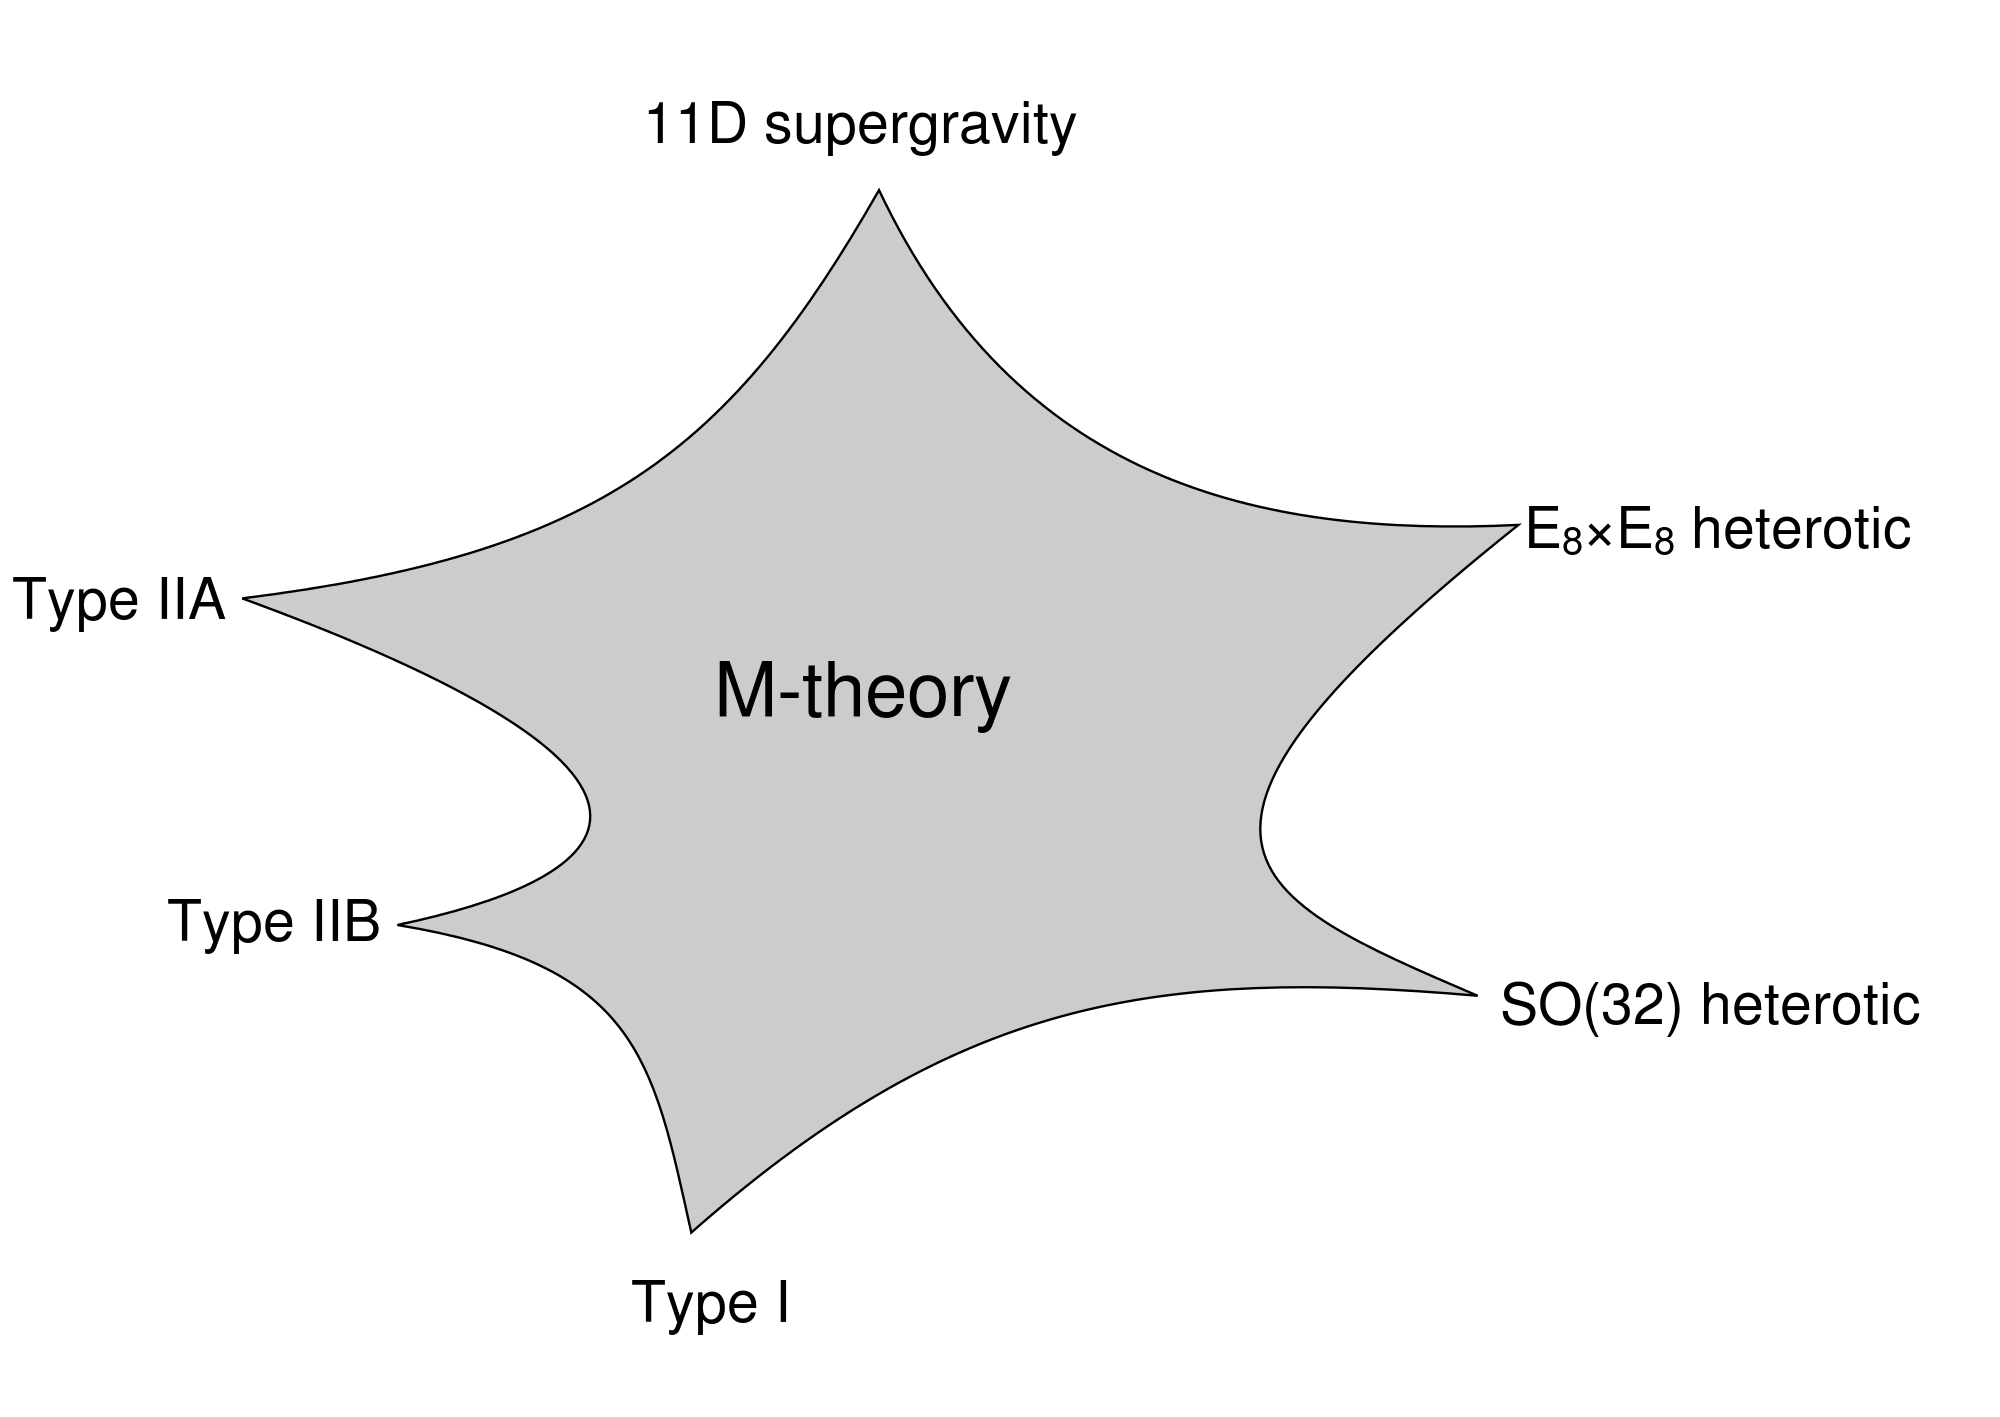
\includegraphics [width=0.5\textwidth]{Mtheory}
\caption{Different types of Superstring Theory}
\label{Mtheory}
\end{figure}

\vspace{1.5em}

In 90's there was the so called ``second superstring revolution'' in which, among other things, Edward Witten proposed that all those different types of superstring theories, were in fact different limits of one unique theory called ``M-Theory'', which the low energy limit leads to eleven dimensional SUGRA. Further work towards this direction, revealed the existence of various dualities and other mechanisms, which relate one theory to another. For instance, one can compactify the eleven dimensional M-Theory in order to obtain type IIA superstring theory, which in turn is related to type IIB theory, under a duality which wraps the IIA string on a circle of radius $R$, called T-duality.

In this project we will work with type II superstring theory.

\section{Type II Superstring Theory}

M theory is comprised of the metric $g_{\mu\nu}$, and an antisymmetric three-form gauge field $A_{\mu\nu\rho}$ with its corresponding four-form field strength $F_{\mu\nu\rho\sigma}$. As we already mentioned, a relation between eleven-dimensional theory and ten-dimensional type IIA theory exists. The way to proceed, is by making the eleventh dimension small, and compactifying it on a circle. There are two different cases that could happen under compactification. Either one of the components of the fields lie along the eleventh dimensions, or the field was completely inside the ten dimensional spacetime, and it retains its form.

\vspace{2em}

\begin{center}
\begin{tabular}{llr}
\toprule
\multicolumn{2}{c}{\:\:\:\:\:\:\:\: M-Theory Compactification} \:\:\:\:\:\:\:\: \\
\midrule
{\small{}}\\
\:\:\:\:\:\:\:\:\:\: $g^{\text{M}}_{\mu\nu}$ $\rightarrow$ $g^{\text{IIA}}_{\mu\nu}$ or $C_{\mu} = g^{\text{M}}_{\mu 11}$    \\\\
\:\:\:\:\:\:\:\: $C^{\text{M}}_{\mu\nu\rho}$ $\rightarrow$ $C^{\text{IIA}}_{\mu\nu\rho}$ or $B_{\mu\nu} = C^{\text{M}}_{\mu\nu11}$ \\\\
\:\:\:\:\:\: $F^{\text{M}}_{\mu\nu\rho\sigma}$ $\rightarrow$ $F^{\text{IIA}}_{\mu\nu\rho\sigma}$ or $H_{\mu\nu\rho} = C^{\text{M}}_{\mu\nu\rho11}$ \\\\
\bottomrule
\end{tabular}
\end{center}

\vspace{2em}

The resulting fields that we obtain out of this process, are the fields of type IIA superstring theory which can be categorised in two sectors of fields. The first one is called ``NS-NS Sector'' and the second is called ``R-R Sector''. In what follows, we will describe the bosonic fields of these two sectors.

The fields of the NS-NS sector can be obtained by acting on the vacuum state with the creation operator $\alpha^{-1}_\mu$. Since we are interested in working in the low energy limit of string theory, we want the mass of the particles to be as low as possible. By choosing to act on the vacuum with two creation operators we manage to get zero-mass particles.

\begin{align} \label{Tasos}
\alpha^{-1}_\mu \alpha^{-1}_\nu \ket{0} = \text{massless particles}
\end{align}

\vspace{0.5em}
In order to express (\ref{Tasos}) in an irreducible way, we split the combination of creation operators to a symmetric part without the trace, to an antisymmetric part and to the trace. The excitations that we get out of this split is the graviton $g_{\mu\nu}$, the antisymmetric 2-form $B_2$ and the dilaton $\phi$ respectively. These three fields form the NS-NS sector.

On the other hand, the R-R sector contains the generalised gauge fields $C_p$. In electrodynamics, the electric charge $e$, couples electrically to the $U(1)$ gauge field as

\begin{align}
S_{\text{el}} = e \int A_1
\end{align}

\vspace{0.5em}
or magnetically to the dual U(1) gauge fields ${\tilde{A}}_1$ as

\begin{align}
S_{\text{el}} = g_{M} \int {\tilde{A}}_1
\end{align}

\vspace{0.5em}
In ten dimensions we are allowed to define a larger number of dual gauge fields $C_p$, where $p=0,1, \ldots$. These gauge fields form the R-R sector.

Type II has a further separation in type IIA and type IIB, depending on the chirality of the gauge fields. More specifically, type IIA contains only non-chiral fields, (i.e. left-right symmetric), while type IIB contains chiral fields. The NS-NS sector is common to both theories, while fields of the R-R sector are categorised as follows 

\vspace{2em}

\begin{center}
\begin{tabular}{llr}
\toprule
\multicolumn{2}{c}{Bosonic Fields - Type II SUGRA} \\
\midrule
NS - NS Sector:  &$g_{\mu\nu}$, $B^{(2)}_{\mu\nu}$, $\phi$ \\\\
R - R Sector (Type IIA):  &$C^{(1)}_{\mu}$, $C^{(3)}_{\mu\nu\rho}$ \\\\
R - R Sector (Type IIB):  &$C^{(0)}$, $C^{(2)}_{\mu\nu}$, $C^{(4)}_{\mu\nu\rho\sigma}$ \\
\bottomrule
\end{tabular}
\end{center}

\vspace{2em}

In what follows we will work with type IIA superstring theory, but the whole procedure can be redone in the framework of type IIB.

\section{Action of Type IIA Superstring Theory}

As we described in the previous section, the fields that constitute type IIA superstring theory are the graviton $g_{\mu\nu}$, the antisymmetric 2-form $B_2$ and the dilaton $\phi$ coming from NS-NS sector, and the gauge fields $C^{(0)}$, $C^{(2)}$ along with their duals $C^{(6)}$, $C^{(8)}$ coming from R-R sector. Now we are ready to define the effective action of Type IIA supergravity which is the low energy limit of Type IIA superstring theory. The action, which is separated into three individuals terms, is of the form:

\begin{align} \label{4.1}
S_{IIA} = S_{NS-NS} + S_{R-R} + S_{CS}
\end{align}

\vspace{0.5em}
Since we are interested to study black holes, the usual tactic is to write down the action in the Einstein frame, in which the Ricci scalar is not multiplied by the dilaton term. In the democratic formulation framework, where all the fields appear in the action, the explicit form of each term is:\footnote{The following notation is used through out this paper:
\begin{equation*}
{|{F}_{n}|}^2 = \frac{1}{n!} g^{\mu_{1}\nu_{1}} g^{\mu_{2}\nu_{2}} \ldots g^{\mu_{n}\nu_{n}} {F}_{\mu_{1} \mu_{2} \ldots \mu_{n}} {F}_{\nu_{1} \nu_{2} \ldots \nu_{n}}
\end{equation*}
\begin{equation*}
{|{F}_{n}|}^2_{\mu\nu} =  \frac{1}{(n-1)!} g^{\mu_{2}\nu_{2}} \ldots g^{\mu_{n-1}\nu_{n-1}} {F}_{\mu \mu_{2} \ldots \mu_{n-1}} {F}_{\nu \nu_{2} \ldots \nu_{n-1}}
\end{equation*}}

\begin{gather}
S_{NS-NS} = \frac{1}{2\kappa^{2}} \int d^{10}x \sqrt{-g} \Big(R - \frac{1}{2} \partial_{\mu} \phi \partial^{\mu} \phi - \frac{1}{2} e^{-\phi} {|H_{3}|}^2 \Big) \label{4.2} \\
S_{R-R} = \frac{1}{2\kappa^{2}} \int d^{10}x \sqrt{-g} \Big( - \frac{1}{2} e^{\frac{3\phi}{2}} {|\tilde{F}_{2}|}^2 - \frac{1}{2} e^{\frac{\phi}{2}} {|\tilde{F}_{4}|}^2 \Big) \label{4.3}\\
S_{CS} = - \frac{1}{4\kappa^{2}} \int B_{2} \wedge \tilde{F}_{4} \wedge \tilde{F}_{4} \label{4.4}
\end{gather}

\vspace{0.5em}
where $H_{3} = dB_{2}$, $F_{n} = dC_{n-1}$ and the tilde fields are

\begin{align} \label{4.5}
\tilde{F}_{2} = F_{2} \qquad \tilde{F}_{4} = F_{4} + C_{1} \wedge H_{3} 
\end{align}

\vspace{0.5em}
following the general rule

\begin{align} \label{4.6}
\tilde{F}_{n} = F_{n} + C_{n-3} \wedge H_{3} 
\end{align}

\vspace{0.5em}
A topological Chern-Simons term in 10 dimensions has also been included.

As in four dimensions, it is convenient to define the dual fields based on the equations of motion. We define the dual field of the antisymmetric $B_{2}$ field to be the 7-form:

\begin{align} \label{4.7}
{H}_7 = e^{-\phi} * {H}_3
\end{align}

and upon employing the following rule:

\vspace{0.5em}
\begin{align} \label{4.8}
{\tilde{F}}_n = {(-1)}^{\frac{(n-1)(n-2)}{2}} e^{\frac{n-5}{2}\phi} * {\tilde{F}}_{10-n}, \qquad n\geq5
\end{align}

\vspace{0.5em}
we define the dual fields of the R-R sector as:

\begin{align} \label{4.9}
{\tilde{F}}_6 = e^{\frac{\phi}{2}} * \tilde{F}_4 \qquad {\tilde{F}}_8 = - e^{\frac{3\phi}{2}} * \tilde{F}_2 
\end{align}

\vspace{0.5em}
Based on (\ref{4.5}) and on the fact that $H_{3} = dB_{2}$ we get the following Bianchi identities:

\begin{align} \label{4.10}
dH_{3} = 0 \qquad d\tilde{F}_{2} = 0 \qquad d\tilde{F}_{4} = H_{3} \wedge \tilde{F}_{2}
\end{align}

\vspace{0.5em}
By varying the action with respect to the gauge fields (see Appendix  \ref{ABC2}) we can derive the equations of motion for $H_3$, ${\tilde{F}_{2}}$ and ${\tilde{F}_{4}}$, where in a compact way they can be written as:

\begin{gather}
d*e^{-\phi} H_3 = \frac{1}{2} \sum_{\text{all fields}} e^{\frac{5-n}{2}\phi} {\tilde{F}_{n-2}} \wedge * {\tilde{F}_{n}} \label{4.11} \\
d*e^{\frac{5-n}{2}\phi}{\tilde{F}_{n}} = e^{\frac{3-n}{2}\phi} *{\tilde{F}_{n+2}} \wedge H_3 \label{4.12}
\end{gather}

\vspace{0.5em}
where in order for these relations to make sense, the dual fields definitions (\ref{4.7}) and (\ref{4.9}) must be used.

Combining the definitions of the dual fields with (\ref{4.7}) and (\ref{4.9}), we can see that the equations of motion of the original fields are the Bianchi identities of the dual fields. We can rewrite everything in a more compact notation as \cite{blaaback2010smeared}

\begin{gather}
dH_3 = 0, \label{4.13} \\
dH_7 = \frac{1}{2} \sum_{\text{all fields}} e^{\frac{5-n}{2}\phi} {\tilde{F}_{n-2}} \wedge * {\tilde{F}_{n}}, \label{4.14} \\
d\tilde{F}_{n} = H_3 \wedge \tilde{F}_{n-2} \label{4.15}
\end{gather}

\section{Einstein Equations for Type IIA Supergravity}

The goal is to repeat the steps that we did in four dimensions, in order to calculate the Smarr formula for type IIA supergravity in 10 dimensions. The Smarr formula (\ref{Smarr}) in 10 dimensions is of the form

\begin{align} \label{4.16}
M = \frac{1}{14\pi G_{10}} \int\limits_{\Sigma} R^{\mu\nu} K_{\mu} d\Sigma_{\nu} + \frac{1}{14\pi G_{10}}  \int\limits_{\partial \Sigma^{\text{h}}} \Big( \nabla^{\mu} K^{\nu} + \Lambda \omega^{\mu\nu} \Big) d\Sigma_{\mu\nu}\end{align}

\vspace{0.5em}
The first step is to find the form of Ricci tensor for the action (\ref{4.1}).

Given (\ref{4.2}) and (\ref{4.3}), we can calculate Einstein equations by varying the action with respect to the metric. As in four dimensions, the Chern-Simons term (\ref{4.4}) is purely topological and subsequently it does not contribute to the Einstein equations.

The variation of the general field ${F}_{n}$ with respect to the metric gives (see Appendix  \ref{ABC2}): 

\begin{align} \label{4.17}
\frac{\delta {|{F}_{n}|}^2}{\delta g_{\mu \nu}} = {|{F}_{n}|}^2_{\mu\nu} 
\end{align}

\vspace{0.5em}
Using (\ref{4.17}), by varying action (\ref{4.1}) with respect to the metric we obtain the following Einstein equations

\begin{align} \label{4.18}
R_{\mu\nu} - \frac{1}{2} g_{\mu\nu} \: R = \:\:\: & \frac{1}{2} \partial_{\mu} \phi \partial_{\nu} \phi - \frac{1}{4} g_{\mu\nu} \partial_{\rho} \phi \partial^{\rho} \phi - \frac{1}{4} e^{-\phi} g_{\mu\nu} {|H_{3}|}^2 \notag \\
&+ \frac{1}{2} e^{-\phi} {{|H_{3}|}^2}_{\mu\nu} - \frac{1}{4} e^{\frac{3\phi}{2}} g_{\mu\nu} {|\tilde{F}_{2}|}^2 + \frac{1}{2} e^{\frac{3\phi}{2}} {{|\tilde{F}_{2}|}^2}_{\mu\nu} \notag \\
&- \frac{1}{4} e^{\frac{\phi}{2}} g_{\mu\nu} {|\tilde{F}_{4}|}^2 + \frac{1}{2} e^{\frac{\phi}{2}} {{|\tilde{F}_{4}|}^2}_{\mu\nu}
\end{align}

\vspace{0.5em}
By contracting the indices, equation (\ref{4.18}) admits

\begin{align} \label{4.19}
R = \frac{1}{2} \partial_{\mu} \phi \partial^{\mu} \phi + \frac{1}{4}e^{-\phi} {|H_{3}|}^2 + \frac{3}{8} e^{\frac{3\phi}{2}} {|\tilde{F}_{2}|}^2 + \frac{1}{8} e^{\frac{\phi}{2}} {{|\tilde{F}_{4}|}^2}
\end{align}

\vspace{0.5em}
Substituting (\ref{4.19}) back to (\ref{4.18}), we finally obtain

\begin{align} \label{4.20}
R_{\mu\nu} = \frac{1}{2} \partial_{\mu} \phi \partial_{\nu} \phi + e^{-\phi} {\{ {H}_{3}\}}^2_{\mu\nu} + e^{\frac{3\phi}{2}} {\{ {\tilde{F}}_{2}\}}^2_{\mu\nu} + e^{\frac{\phi}{2}} {\{ {\tilde{F}}_{4}\}}^2_{\mu\nu}
\end{align} 

\vspace{0.5em}
where in the last equation the following notation has been used:

\begin{align} \label{4.21}
{\{ {F}_{n}\}}^2_{\mu\nu} = \frac{1}{2} \Big( {|{F}_{n}|}^2_{\mu\nu} - \frac{(n-1)}{8} g_{\mu\nu} {|{F}_{n}|}^2 \Big)
\end{align}

\vspace{0.5em}
As in chapter 3, by manipulating the definition of the dual fields (\ref{4.7}) and (\ref{4.9}) we can prove the following relation between the fields and their duals

\begin{align} \label{4.22}
{{|F}_n|}^2_{\mu\nu} = e^{\pm (n-5)\phi} \Big(|F_{10-n}|^2_{\mu\nu} - g_{\mu\nu} |F_{10-n}|^2 \Big)
\end{align}

\vspace{0.5em}
where $(+)$ stands for R-R sector and $(-)$ for NS-NS sector.

Solving with respect to the metric equation (\ref{4.22}), Einstein equations (\ref{4.20}), can be rewritten as

\begin{align} \label{4.23}
R_{\mu\nu} = & \frac{1}{2} \partial_{\mu} \phi \partial_{\nu} \phi + \frac{3}{8} e^{-\phi} {|H_{3}|}^2_{\mu\nu} + \frac{1}{8} e^{\phi} {|H_{7}|}^2_{\mu\nu} + \frac{7}{16} e^{\frac{3\phi}{2}}|{\tilde{F}_{2}|}^2_{\mu\nu} \notag \\ 
& + \frac{1}{16} e^{-\frac{3\phi}{2}} |{\tilde{F}_{8}|}^2_{\mu\nu} + \frac{5}{16} e^{\frac{\phi}{2}} |{\tilde{F}_{4}}|^2_{\mu\nu} + \frac{3}{16} e^{-\frac{\phi}{2}} |{\tilde{F}_{6}}|^2_{\mu\nu}
\end{align}

\vspace{0.5em}
As we already showed before, scalar fields do not contribute at all to the bulk integral, hence the dilaton part does not appear in Smarr formula. By keeping this in mind, we can use Ricci tensor of the form (\ref{4.23}) and the definitions of the dual fields (\ref{4.7}) and (\ref{4.9}) in order to write Smarr formula in an elegant way in terms of differential forms as (see Appendix \ref{ABC1})  

\begin{align} \label{4.24}
M &= \frac{1}{224 \pi G_{10}} \int\limits_{\Sigma} \Big( -6 i_K H_3 \wedge H_7 - 2 i_K H_7 \wedge H_3 - 7 i_K \tilde{F}_2 \wedge \tilde{F}_8  \\ \notag
& \:\:\:\:\:\:\:\:\:\:\:\:\:\:\:\:\:\:\:\:\:\:\:\:\:\:\:\:\:\:\: + i_K \tilde{F}_8 \wedge \tilde{F}_2 + 5 i_K \tilde{F}_4 \wedge \tilde{F}_6 - 3 i_K \tilde{F}_6 \wedge \tilde{F}_4 \Big) \\ \notag
&+ \frac{1}{14\pi G_{10}}  \int\limits_{\partial \Sigma^{\text{h}}} \Big( \nabla^{\mu} K^{\nu} + \Lambda \omega^{\mu\nu} \Big) d\Sigma_{\mu\nu}
\end{align}

\vspace{0.5em}
Once again in order to proceed we need to calculate the contraction of the Killing vector with the various fields.

\section{Invariances}

At this point we make the same assumption we did in the four dimensional case. Namely, that the matter fields of the theory respect the symmetries of the metric. Therefore, assuming that there is an isometry generated by a Killing vector field $K$, we get the following equations

\begin{gather}
\mathcal{L}_{K} \phi = 0 \label{4.25} \\
\mathcal{L}_{K} H_{3} = 0 \label{4.26} \\ 
\mathcal{L}_{K} H_{7} = 0 \label{4.27} \\
\mathcal{L}_{K} \tilde{F}_{n} = 0, \:\:\:\:\:\:  n=2,4,6,8 \label{4.28}
\end{gather}

\vspace{0.5em}
Using Cartan's magic formula (\ref{3.19}), we can manipulate equations (\ref{4.25}) to (\ref{4.28}) in the same manner we did in chapter 3. Namely, as we already mentioned, we anticipate no contribution from scalar fields. Indeed, (\ref{4.25}) for the dilaton admits

\begin{align} \label{4.29}
i_{K} (d \phi) = 0
\end{align}

\vspace{0.5em}
Equation (\ref{4.26}) for $H_{3}$ produces straightforwardly that

\begin{align} \label{4.30}
i_{K} H_{3} = \Lambda_{2} + d\lambda_{1}
\end{align}

\vspace{0.5em}
where $\Lambda_{2}$ is a harmonic form and $d\lambda_{1}$ is an exact form.

\vspace{0.5em}
In the same way, one can manipulate equations (\ref{4.28}), and the final result can be written in a compact way as

\begin{align} \label{4.31}
i_{K} \tilde{F}_{n} = \Omega_{n-1} \wedge e^{B_2} + d\omega_{n-2} \wedge e^{B_2} - \Lambda_{2} \wedge C_{n-3}
\end{align}

\vspace{0.5em}
where $\Omega_{n}$ are harmonic n-forms and $d\omega_{n}$ are exact n-forms originated by the R-R sector. Equation (\ref{4.30}) is written in terms of polyforms. One can expand (\ref{4.30}) according to the following formula

\begin{align} \label{4.32}
A_p \wedge e^{B_2} = A_p + A_{p-2} \wedge B_2 + \frac{1}{2} A_{p-4} \wedge B_2 \wedge B_2 + \ldots 
\end{align}

\vspace{0.5em}
Finally by making use of (\ref{4.30}) and (\ref{4.31}), we can manipulate (\ref{4.27}) and the final result is of the form

\begin{align} \label{4.33}
i_{K} \tilde{H}_{7} = & - (\Omega_{5} + d\omega_{4}) \wedge C_1 + \Omega_{3} + d\omega_{2} \wedge (C_3 - B_2 \wedge C_1) \notag \\
& - (\Omega_{1} + d\omega_{0}) \wedge (C_5 - B_2 \wedge C_3 + \frac{1}{2} B_2 \wedge B_2 \wedge C_1) \notag \\
& + (\Lambda_2 + d\lambda_1) \wedge C_1 \wedge C_3 + \Lambda_6 + d\lambda_5
\end{align}

\vspace{0.5em} 
where $\Lambda_6$ and $d\lambda_5$ are the harmonic and the exact forms coming from the dual fields of $B_2$, i.e the NS-NS sector.

\section{Smarr Formula for Type IIA Supergravity}

Once we calculated all the contractions of the Killing vectors with the fields, we are know ready to calculate Smarr formula in 10 dimensions, by substituting equations (\ref{4.29}) - (\ref{4.31}) and equation (\ref{4.33}) back to Smarr formula (\ref{4.24}). 

As we already mentioned in four dimensional case, exact forms do not contribute at all to the bulk and they can be moved to boundaries integrals via Stokes' theorem. Once again, we make the assumption that all the corresponding terms are small at infinity, hence, the LHS of Smarr formula remains the same. Finally,  after removing the event horizon integral, we obtain the final ten dimensional Smarr formula for type IIA supergravity which is

\begin{align} \label{4.34}
M = &\int\limits_{\Sigma} \Lambda_2 \wedge f(\text{fields}) + \Lambda_6 \wedge H^{*}_3 + \sum_{n}^{1,3,5,7} \Omega_n \wedge \Big( \tilde{F}^{*}_{9-n} + H^{*}_3 \wedge C^{*}_{6-n}  \Big) \wedge e^{B_2}
\end{align}

\vspace{0.5em} 
where the function f is equal to:

\begin{align} \label{4.35}
f = H^{*}_7 - \tilde{F}^{*}_{6} \wedge C^{*}_{1} - \tilde{F}^{*}_{4} \wedge C^{*}_{3} -  \tilde{F}^{*}_{2} \wedge C^{*}_{5} + C^{*}_{1} \wedge C^{*}_{3} \wedge H^{*}_3
\end{align}

\vspace{0.5em} 
and we redefined the fields in the following way:

\begin{gather}
C^{*}_{n} = (-1)^{\frac{5-n}{2}} C_n \label{4.36} \\
H^{*}_n = (-1)^{\frac{5-n}{2}} (n-1) H_n \label{4.37} \\
F^{*}_{n} = (-1)^{\frac{10-n}{2}} (n-1) F_n \label{4.38}
\end{gather}

\vspace{0.5em} 
Our final Komar mass (\ref{4.34}) is a higher dimensional analog of the Komar mass (\ref{3.29}) in 4 dimensions. The extra dimensions of our theory made the ten dimensional result of Komar mass (\ref{4.35}) to include harmonic forms of various dimensions. The latter provides us with more freedom on choosing the topology of the spacetime without getting a zero mass.

In the case, for instance, where one restricts themselves to work only with simply connected topological space, hence trivial first cohomology group, we get as a result that a harmonic 1-form cannot exist, subsequently $\Omega_1 = 0$. 

On top of that, we could also assume that our space has a trivial second cohomology group, which would admit a vanishing harmonic 2-form, hence $\Lambda_2$ also could not exist. However, even then, we would have been left with a plethora of non-vanishing harmonic forms that deter the mass from vanishing, since our topological space could have non-trivial cohomology groups $H^n(M)$ for $n=3,5,6,7$.

Therefore, we showed that adding extra dimensions to our theory, involves more cohomology groups, and saves the Komar mass from vanishing. One does not necessarily need to assume ten dimensions, in order to get an interesting result. The same outcome can been achieved even in five \cite{gibbonsglobal} or six dimensions \cite{de2015structure}. Once again, the latter underlines the difficulty of finding microstate geometries in four dimensions.

\chapter{Conclusion}

The objective of the present thesis was to verify that there is another way, apart from black holes, to support mass from gravitational collapse. As we mentioned, these new solutions of Einstein Equations, called microstate geometries, are time-independent, horizonless, and smooth meaning that they carry no singularity. Moreover, we verified that, in order for microstate geometries to support mass, they should also have non-trivial cohomology groups. Finally, we extended this mechanism to asymptotically non-flat AdS spacetime, and we showed the need of a way to overcome the divergence, coming from the cosmological constant.

Our four-dimensional result suggests that if we restrict ourselves to work with simply connected topological spaces, there is no way to obtain microstate geometries. The way to overcome this problem relies on finding microstate geometries in higher dimensional spaces. The first solution that was studied, with a non-vanishing result is the five-dimensional case, which was originally published by Gibbons and Warner in 2014 \cite{gibbonsglobal}. They introduced a mechanism containing a Komar Integral and the Smarr formula, and this was used in the present thesis, and more specifically in chapters 3 and 5. We pointed that the pioneering idea that Gibbons and Warner introduced, was to remove the event horizon integral of Smarr formula and to focus only on the topological integral. Earlier one treated the Smarr formula in the opposite way, by assuming that there is no topology, and the whole contribution comes from the event horizon.

Moreover, a paper published in 2015, \cite{de2015structure} dealt with the six-dimensional case, while at the same time, another paper \cite{haas2014smarr} was published, in the framework of the eleven-dimensional supergravity. A further relation between solutions was also established, since upon Calabi-Yau compactification of the eleven-dimensional result provided us with the five-dimensional result, originally obtained by Gibbons and Warner \cite{gibbonsglobal}.
 
In the present thesis, we studied ten dimensions, in the general framework of type IIA superstring theory. Based on the studies \cite{gibbonsglobal,de2015structure,haas2014smarr}, we speculated that the extra dimensions would provide us with a non-zero result, even in the case of simply connected topological spaces. Indeed, the harmonic forms that we got in the final result, were of various dimensions, which gave us freedom to work with the associated cohomology groups.

As far as the extension in AdS spacetime is concerned, during the last years, myriads of studies were published. In particular, Brown and York introduced the idea of the quasilocal stress-energy tensor \cite{brown1993quasilocal,balasubramanian1999stress}. Their proposal was to redefine the stress-energy tensor at infinity including the extrinsic curvature of the spacetime, and an extra counter-term which would cancel the divergence coming from the extrinsic curvature. Another example, consists of the gravitational Hamiltonian formalism, introduce by Hawking and Horowitz \cite{hawking1996gravitational}. As the name indicate, this is an additional way to describe gravity, using a Hamiltonian formalism, which could be used to treat the divergence. 

This thesis, however, dealt with the divergence coming from the cosmological constant, by introducing the Killing Potential. As we showed, the latter cancels the divergence of the Komar Integral at infinity, but it also fits well with the Smarr formula, since it treats the divergence in the bulk as well.

It would be of great interest for future studies to apply to some specific geometries, such as the LLM geometries $AdS_5 \times S_5$, or more general geometries of the form $AdS_p \times S_q$ in the result we obtained in type IIA in ten dimensions (\ref{4.34}). (For general review of these geometris see \cite{lin2004bubbling,yamaguchi2007bubbling}). Our anticipation is to find a relation between the mass and the charges of the brains that were used in order to build the black hole. Furthermore, it would be interesting to obtain the six- and five-dimensional result by compactifying our own result. That way, we would have a complete catalogue of all the different results.

Last but not least, concerning the AdS divergence, one could try to apply one of the above-mentioned suggestions (i.e, quasilocal stress-energy tensor and gravitational Hamiltonian formalism) when topology is present.

\appendix
\chapter{Differential Forms \& Conventions} \label{AB}

A differential $p$-form is defined as

\begin{align}
A_p = \frac{1}{p!} A_{\mu_{1} \ldots \mu_{p}} dx^{\mu_{1}} \wedge \ldots \wedge dx^{\mu_{p}}
\end{align}

\vspace{0.5em}
where the wedge product ($\wedge$) denotes the antisymmetry

\begin{align} \label{a}
dx^{\mu} \wedge dx^{\nu} = - dx^{\nu} \wedge dx^{\mu}
\end{align}

\vspace{0.5em}
Hence, a $0$-form is just an function, an $1$-form could be a $U(1)$ gauge field $A = A_\mu dx^\mu$, a $2$-form could be the associated field strength of a gauge field $F=\frac{1}{2} F_{\mu\nu} dx^\mu dx^\nu$ etc.

Relation (\ref{a}) manifests the following algebra for two forms

\begin{align} \label{a}
A_p \wedge B_q = - (-1)^{pq} B_q \wedge A_p
\end{align}

\vspace{0.5em}
Another useful tool in differential forms is the exterior derivative ($d$) which is the way to get the derivative of forms. Exterior derivative, obeys Leibniz rule and acts on a form in the following way

\begin{align}
dA_p = \frac{1}{p!} \partial_{\nu }A_{\mu_{1} \ldots \mu_{p}} dx^{\nu} \wedge dx^{\mu_{1}} \wedge \ldots \wedge dx^{\mu_{p}}
\end{align}

\vspace{0.5em}
A differential form is called closed if $dA_p = 0$, and it is called exact if it can be written as the exterior derivative of another (p-1) form, i.e: $A_p = dB_{p-1}$. An exact form is always closed, while the reverse does not necessarily hold.  

The Hodge dual operator (*) is a map which sends a $p$-form to a $(d-p)$-form, where $d$ stands the dimensions of the manifold, according to the following rule

\begin{align}
*A_p = \frac{1}{p!}  \frac{1}{(d-p)!} A_{\mu_{1} \ldots \mu_{p}} \epsilon^{\mu_{1} \ldots \mu_{p}}_{\:\:\:\:\:\:\:\:\:\:\:\: \nu_{p+1} \ldots \nu_{d}} dx^{\nu_{p+1}} \wedge \ldots \wedge dx^{\nu_{d}}
\end{align}

\vspace{0.5em}
where $\epsilon_{\mu_{1} \ldots \mu_{d}} = \sqrt{-g} \varepsilon_{\mu_{1} \ldots \mu_{d}}$ and $\varepsilon$ is the  Levi-Civita symbol which in $d$ dimensions obeys the following convention

\begin{align}
\varepsilon_{0 1 \ldots d-1} = 1
\end{align}

\vspace{0.5em}
and it is fully antisymmetric $\varepsilon_{\mu_{1} \ldots \mu_{p}} = \varepsilon_{[\mu_{1} \ldots \mu_{p}]}$. For the contraction of the $\epsilon$ tensor holds:

\begin{align}
\epsilon_{\mu_{1} \ldots \mu_{p} \mu_{p+1} \ldots \mu_{d}} \epsilon^{\mu_{1} \ldots \mu_{p} \nu_{p+1} \ldots \nu_{d}} = (-1)^t p! (d-p)! \delta_{\mu_{p+1} \ldots \mu_{d}}^{\nu_{p+1} \ldots \nu_{d}}
\end{align}

\vspace{0.5em}
where $t$ is the number of the timelike components of the spacetime. $\delta_{\mu_{1} \ldots \mu_{p}}^{\nu_{1} \ldots \nu_{p}}$ is the generalised Kronecker delta which is defined by the following relation

\begin{align}
\delta^{\mu_{1} \ldots \mu_{p}}_{\nu_{1} \ldots \nu_{p}}=
\begin{cases}
+1 & \text{if $\nu_{1} \ldots \nu_{p}$ are an even permutation of $\mu_{1} \ldots \mu_{p}$}\\
-1 & \text{if $\nu_{1} \ldots \nu_{p}$ are an odd permutation of $\mu_{1} \ldots \mu_{p}$}\\
0 & \text{in any other case}
\end{cases}
\end{align}

\vspace{0.5em}
Generalized Kronecker delta has the following useful property

\begin{align}
\delta^{\mu_{1} \ldots \mu_{p}}_{\nu_{1} \ldots \nu_{p}} = \sum_{n=1}^{p} (-1)^{n+p} \delta^{\mu_{p}}_{\nu_{n}} \delta^{\mu_{1} \ldots \mu_{n} \ldots \tilde{\mu_{p}}}_{\nu_{1} \ldots {\tilde{\nu}}_{n} \ldots \mu_{p}} 
\end{align}

\vspace{0.5em}
where the tilde notation means that the particular term should be left out form the sequence.

Generalized Kronecker delta can act on a tensor in the following way

\begin{align}
\delta^{\mu_{1} \ldots \mu_{p}}_{\nu_{1} \ldots \nu_{p}} \omega^{\nu_{1} \ldots \nu_{p}}  = p! \omega^{[\mu_{1} \ldots \mu_{p}]}  \\
\delta^{\mu_{1} \ldots \mu_{p}}_{\nu_{1} \ldots \nu_{p}} \omega_{\mu_{1} \ldots \mu_{p}}  = p! \omega_{[\nu_{1} \ldots \nu_{p}]} 
\end{align}

\vspace{0.5em}
Finally, another useful formula is the contraction of generalized Kronecker delta with itself which produces

\begin{align}
\delta^{\mu_{1} \ldots \mu_{p}}_{\nu_{1} \ldots \nu_{p}} \delta_{\rho_{1} \ldots \rho_{p}}^{\nu_{1} \ldots \nu_{p}}  = p! \delta^{\mu_{1} \ldots \mu_{p}}_{\rho_{1} \ldots \rho_{p}}
\end{align}

\vspace{0.5em}
Hodge dual satisfies the following properties

\begin{align}
*A_p \wedge B_p = *B_p \wedge A_p \\
**A_p = (-1)^{p(d-p) + t} A_p
\end{align}

\vspace{0.5em}
Regarding integration of differential forms, Stokes' theorem can be written in an elegant way using forms as

\begin{align}
\int\limits_{\Sigma} dA_p =  \int\limits_{\partial \Sigma} A_p
\end{align}

\vspace{0.5em}
where $\Sigma$ denotes the spatial components of the manifold and $\partial \Sigma$ is a hupersuface boundary which includes $\Sigma$. In the case where manifold $\Sigma$ has also an inner boundary $\partial \Sigma^{\text{inner}}$ beside from an outer boundary $\partial \Sigma^{\text{outter}}$, Stokes' theorem becomes

\begin{align}
\int\limits_{\Sigma} dA_p =  \int\limits_{\partial \Sigma^{\text{outter}}} A_p - \int\limits_{\partial \Sigma^{\text{inner}}} A_p
\end{align}

\chapter{Cohomology} \label{ABC}

Homology, which is a commutative alternative to homotopy, is a tool of algebraic topology which associates a sequence of abelian groups to a topological space. The dual of homology, is called cohomology. We define the r-cohomology group of a topological space, to be the quotient group of all closed $r$-forms (i.e $dA=0$) modulo the exact $r$-forms (i.e $A=dB$).

\begin{align}
H^r(M) = \frac{Z^r(M)}{B^r(M)}
\end{align}

\vspace{0.5em}

where $H^r(M)$ is the r cohomology of the manifold $M$. $Z^r(M)$ is called ``the group of cocycles'' and it contains all the $r$-forms which are closed, and $B^r(M)$ is called ``the group of coboundaries'' and it contains all the r-forms that are exact. 

Cohomology gives us the information of which forms are allowed by the topology and which are not. For instance, a trivial cohomology, (i.e $H^r(M)=0$ where 0 stand for the unit element of the commutative theory), admits that all the closed forms are exact.


\chapter{Derivation of Various Formulas}

\section{Action in Forms and in Index Notation}  \label{ABC1}

One can interchange between an action in terms of form notation and in terms of notation with indices. The following proof applies between the two notations

\begin{align}
*F_p \wedge F_p &= \frac{1}{p!} F_{\mu_{1} \ldots \mu_{p}} \frac{1}{(d-p)! p!} F^{\nu_{1} \ldots \nu_{p}} \sqrt{-g} \epsilon_{\nu_{1} \ldots \nu_{p} k_{p+1}k_{d}} dx^{{\mu}_1} \wedge \ldots \wedge dx^{{\mu}_p} \wedge dx^{{k}_{p+1}} \wedge \ldots \wedge dx^{{k}_{d}} \notag \\
& = \frac{1}{p!} F_{\mu_{1} \ldots \mu_{p}} \frac{1}{(d-p)! p!} F^{\nu_{1} \ldots \nu_{p}} \sqrt{-g} \epsilon_{\nu_{1} \ldots \nu_{p} k_{p+1}k_{d}} \epsilon^{\mu_{1} \ldots \mu_{p} k_{p+1}k_{d}} d^dx\notag \\
& = \frac{1}{p!} F_{\mu_{1} \ldots \mu_{p}} \frac{1}{\cancel{(d-p)!} p!} F^{\nu_{1} \ldots \nu_{p}} \cancel{(d-p)!} {\delta{_{\nu_{1} \ldots \nu_{p}}}^{\mu_{1} \ldots \mu_{p}}} \sqrt{-g}d^dx\notag \\
& = \frac{1}{p!} F_{\mu_{1} \ldots \mu_{p}} \frac{1}{\cancel{p!}} \cancel{p!} F^{[\nu_{1} \ldots \nu_{p}]} \sqrt{-g}d^dx\notag \\
& = \frac{1}{p!} F_{\mu_{1} \ldots \mu_{p}} F^{\nu_{1} \ldots \nu_{p}} \sqrt{-g}d^dx\notag \\
& = \frac{1}{p!} g^{\mu_{1}\nu_{1}} \ldots g^{\mu_{p}\nu_{p}} F_{\mu_{1} \ldots \mu_{p}} F^{\nu_{1} \ldots \nu_{p}} \sqrt{-g}d^dx \notag \\
&= \frac{1}{p!} F_{\mu_{1} \ldots \mu_{p}} F^{\mu_{1} \ldots \mu_{p}} \sqrt{-g}d^dx \notag \\
\end{align}

\section{Variation of Field Strength with Respect to the Gauge Fields} \label{ABC2}

In terms of forms, the variation of the field strength $F$ with respect to the gauge field $C$, can be written as

\begin{align}
\delta_C \int F_p \wedge *F_p &= \delta_C \int dC_{p-1} \wedge * dC_{p-1} \notag \\
&= \int d\delta_C C_{p-1} \wedge * dC_{p-1} + dC_{p-1} \wedge * d\delta_C C_{p-1} \notag \\
&= \int d\delta_C C_{p-1} \wedge * dC_{p-1} + d \delta_C C_{p-1} \wedge * dC_{p-1} \notag \\
&= 2 \int d\delta_C C_{p-1} \wedge * dC_{p-1} \notag \\
&= 2 \Big[ \delta_C C_{p-1} \wedge * dC_{p-1} \Big]_{\text{boundaries}} - 2 \int \delta_C C_{p-1} \wedge d * dC_{p-1} \notag \\
&= \int \delta_C C_{p-1} \wedge (- 2 d * dC_{p-1})
\end{align}

\vspace{0.5em}
Hence

\begin{align}
\delta_C \int F_p \wedge *F_p = \int \delta_C C_{p-1} \wedge (- 2 d * F_p) 
\end{align}

\vspace{0.5em}
Same manipulations can prove the following relation between $F_p$ and an abstract form $A_p$
 
\begin{align}
\delta_C \int A_p \wedge *F_p = \delta_C \int F_p \wedge *A_p = \int \delta_C C_{p-1} \wedge (-d * A_p) 
\end{align}

\clearpage

\section{Variation of Field Strength with Respect to the Metric} \label{ABC3}

In order to calculate Einstein equation out of a given action, we need to vary the latter with respect to the metric. By making use of the following notation

\begin{gather}
{|{F}_{n}|}^2 = \frac{1}{n!} g^{\mu_{1}\nu_{1}} g^{\mu_{2}\nu_{2}} \ldots g^{\mu_{n}\nu_{n}} {F}_{\mu_{1} \mu_{2} \ldots \mu_{n}} {F}_{\nu_{1} \nu_{2} \ldots \nu_{n}} \\
{|{F}_{n}|}^2_{\mu\nu} =  \frac{1}{(n-1)!} g^{\mu_{2}\nu_{2}} \ldots g^{\mu_{n-1}\nu_{n-1}} {F}_{\mu \mu_{2} \ldots \mu_{n-1}} {F}_{\nu \nu_{2} \ldots \nu_{n-1}}
\end{gather}

the variation of the general field strength $|F_{n}|$ produces:

\begin{align}
\delta_g {|{F}_{n}|}^2 &= \delta_g \Big( \frac{1}{n!} g^{\mu_{1}\nu_{1}} \ldots g^{\mu_{n}\nu_{n}} F_{\mu_{1} \ldots \mu_{n}} F_{\nu_{1} \ldots \nu_{n}} \Big) \notag \\
&= \frac{1}{n!} \Big( \delta_g g^{\mu_{1}\nu_{1}} \ldots g^{\mu_{n}\nu_{n}} F_{\mu_{1} \ldots \mu_{n}} F_{\nu_{1} \ldots \nu_{n}} + \ldots + g^{\mu_{1}\nu_{1}} \ldots \delta_g  g^{\mu_{n}\nu_{n}} F_{\mu_{1} \ldots \mu_{n}} F_{\nu_{1} \ldots \nu_{n}}  \Big) \notag\\
&= \frac{1}{n!} n \delta_g g^{\mu_{1}\nu_{1}} \ldots g^{\mu_{n}\nu_{n}} F_{\mu_{1} \ldots \mu_{n}} F_{\nu_{1} \ldots \nu_{n}} \notag\\
&= \Big( \frac{1}{n-1} g^{\mu_{2}\nu_{2}}  \ldots g^{\mu_{n}\nu_{n}} F_{\mu_{1} \ldots \mu_{n}} F_{\nu_{1} \ldots \nu_{n}} \Big) \delta_g g^{\mu_{1}\nu_{1}} \notag\\
& = \delta_g g^{\mu_{1}\nu_{1}} {|{F}_{n}|}^2_{\mu_{1}\nu_{1}} \notag
\end{align}

\vspace{0.5em}
Therefore

\begin{align} \label{metric}
\frac{\delta {|{F}_{n}|}^2}{\delta g^{\mu \nu}} = {|{F}_{n}|}^2_{\mu\nu} 
\end{align}

\bibliographystyle{unsrt}
\bibliography{Citations}
\end{document}

